\documentclass[12pt, a4paper]{article}

% ─── Packages ───────────────────────────────────────────────
\usepackage[utf8]{inputenc}
\usepackage[T1]{fontenc}
\usepackage{lmodern}
\usepackage[margin=1in]{geometry}
\usepackage{graphicx}
\usepackage{booktabs}
\usepackage{amsmath, amssymb}
\usepackage{hyperref}
\usepackage{float}
\usepackage{caption}
\usepackage{subcaption}
\usepackage{enumitem}
\usepackage{xcolor}
\usepackage{titlesec}
\usepackage{fancyhdr}
\usepackage{setspace}
\usepackage{longtable}
\usepackage{array}
\usepackage{multirow}
\usepackage{tabularx}

% ─── Page style ─────────────────────────────────────────────
\pagestyle{fancy}
\fancyhf{}
\fancyhead[L]{\small Honours Project Report}
\fancyhead[R]{\small Ablation Zone Prediction}
\fancyfoot[C]{\thepage}
\renewcommand{\headrulewidth}{0.4pt}

% ─── Hyperref setup ─────────────────────────────────────────
\hypersetup{
    colorlinks=true,
    linkcolor=blue!70!black,
    citecolor=blue!70!black,
    urlcolor=blue!70!black
}

% ─── Spacing ────────────────────────────────────────────────
\onehalfspacing

% ─── Graphics path ──────────────────────────────────────────
\graphicspath{{plots/}}

% ─── Title ──────────────────────────────────────────────────
\title{
    \vspace{-1cm}
    \textbf{\LARGE AI/ML-Based Predictive Model for Ablation Zone Estimation in Tumor Treatment}\\[0.8em]
    \large Honours Project Report
}
\author{}
\date{}

% ═════════════════════════════════════════════════════════════
\begin{document}

\maketitle
\thispagestyle{fancy}

% ─── Table of Contents ──────────────────────────────────────
\tableofcontents
\newpage

% ═════════════════════════════════════════════════════════════
\section{Introduction}
\label{sec:introduction}

\subsection{Background}
\label{sec:background}

Cancer remains one of the leading causes of morbidity globally. Minimally invasive thermal ablation techniques --- particularly \textbf{Microwave Ablation (MWA)} --- have emerged as promising alternatives to traditional surgery for the treatment of solid tumors in organs such as the liver, lung, kidney, and adrenal glands. MWA works by delivering electromagnetic energy through interstitial antennas to heat and destroy cancerous tissue, creating a region of necrosis known as the \textbf{ablation zone}.

The shape and dimensions of this ablation zone are critically important: the zone must be large enough to completely cover the tumor while minimizing damage to surrounding healthy tissue. Currently, clinicians rely on a combination of clinical experience, manufacturer-provided ablation charts, and computational simulations (such as Finite Element Method models) to estimate the ablation zone prior to treatment. These approaches are either time-consuming, require specialized software, or fail to generalize across different antenna designs and operating conditions.

\subsection{Problem Statement}
\label{sec:problem-statement}

\begin{quote}
\textit{Develop an AI/ML-based predictive model that accurately estimates the ablation zone produced during tumor treatment using combined hyperthermia and irreversible electroporation parameters, enabling faster and more accurate treatment planning while minimizing damage to surrounding healthy tissues.}
\end{quote}

The central challenge is predicting the \textbf{dimensions of the ablation zone} (diameter, length, volume) from the treatment parameters (input power, duration, antenna type) without requiring computationally expensive physics-based simulations.

\subsection{Objectives}
\label{sec:objectives}

\begin{enumerate}
    \item Collect and curate ablation zone data from published experimental and simulation studies.
    \item Perform comprehensive exploratory data analysis to understand feature relationships.
    \item Engineer meaningful features from raw treatment parameters.
    \item Train and evaluate multiple ML regression models for ablation zone prediction.
    \item Compare model performance and identify the best-performing approach.
    \item Build an interactive prediction system for clinical decision support.
\end{enumerate}

\subsection{Scope of Work}
\label{sec:scope}

This project focuses on \textbf{microwave ablation} data collected from 30+ published research papers spanning 2004--2025. The dataset includes both \textbf{experimental} (ex vivo/in vivo) and \textbf{simulation} (FEM/computational) data across 15+ antenna types and a variety of power levels and treatment durations.

% ═════════════════════════════════════════════════════════════
\section{Literature Review}
\label{sec:literature-review}

\subsection{Microwave Ablation in Tumor Treatment}
\label{sec:mwa}

Microwave ablation employs electromagnetic waves (typically at 915\,MHz or 2.45\,GHz) to induce dielectric heating in biological tissue. Key treatment parameters include:

\begin{itemize}
    \item \textbf{Input Power} (W): Energy delivered to the tissue via the antenna.
    \item \textbf{Treatment Duration} (minutes): Time of energy application.
    \item \textbf{Antenna Design}: Determines the spatial distribution of the electromagnetic field.
    \item \textbf{Frequency}: Operating frequency of the microwave system.
\end{itemize}

The resulting ablation zone is characterized by its \textbf{diameter} (or width), \textbf{length} (longitudinal extent), and overall \textbf{shape} (spherical vs.\ ellipsoidal), which is quantified by the \textbf{sphericity index} (diameter/length ratio).

Several antenna designs have been developed for MWA, including monopole, dipole, dual-slot, triaxial, floating-sleeve, and helical dipole antennas. Each design produces distinct ablation zone geometries based on the specific absorption rate (SAR) pattern it creates.

\subsection{Machine Learning in Medical Treatment Planning}
\label{sec:ml-medical}

Machine learning has been increasingly applied to medical treatment planning, including:

\begin{itemize}
    \item Radiation therapy dose prediction using deep learning.
    \item Surgical outcome prediction using ensemble methods.
    \item Drug response prediction using random forests and neural networks.
    \item Temperature prediction during thermal ablation using deep learning (e.g., the Triple Coaxial-Half-Slot antenna study, 2021).
\end{itemize}

For structured tabular data with limited sample sizes, \textbf{tree-based ensemble methods} (Random Forest, Gradient Boosting) consistently outperform deep learning approaches. This is supported by extensive benchmarking studies and is particularly relevant to our dataset.

\subsection{Existing Approaches \& Research Gap}
\label{sec:research-gap}

Most existing ablation zone prediction methods rely on:

\begin{enumerate}
    \item \textbf{Physics-based simulations} (FEM/FDTD): Accurate but computationally expensive (hours per case).
    \item \textbf{Manufacturer lookup tables}: Quick but limited to specific antenna--power--time combinations.
    \item \textbf{Empirical formulas}: Simple but poor generalization across antenna designs.
\end{enumerate}

\textbf{Research Gap:} There is no comprehensive ML-based predictive model that generalizes across multiple antenna types, power levels, and treatment durations using aggregated data from multiple published studies. This project addresses this gap.

% ═════════════════════════════════════════════════════════════
\section{Dataset Description \& Exploratory Data Analysis}
\label{sec:eda}

\subsection{Data Sources}
\label{sec:data-sources}

Data was curated from two primary categories:

\begin{table}[H]
\centering
\caption{Summary of data sources.}
\label{tab:data-sources}
\begin{tabular}{@{}llll@{}}
\toprule
\textbf{Dataset} & \textbf{Samples} & \textbf{Source Type} & \textbf{Papers} \\
\midrule
Experimental Data & 222 & Ex vivo / In vivo measurements & $\sim$25 papers (2004--2025) \\
Simulated Data    & 104 & FEM / Computational models     & $\sim$15 papers (2009--2025) \\
\midrule
\textbf{Combined Total} & \textbf{326} & Mixed & \textbf{30+ papers} \\
\bottomrule
\end{tabular}
\end{table}

\subsection{Raw Data Structure}
\label{sec:raw-data}

Each data entry contains the fields shown in Table~\ref{tab:raw-data}.

\begin{table}[H]
\centering
\caption{Raw data columns and availability.}
\label{tab:raw-data}
\begin{tabular}{@{}p{4.5cm}p{7cm}l@{}}
\toprule
\textbf{Column} & \textbf{Description} & \textbf{Availability} \\
\midrule
\texttt{PAPERS \& REFERENCES}      & Source paper citation and antenna details          & 100\%  \\
\texttt{INPUT POWER}               & Applied microwave power (e.g., ``50W'', ``100 W'')  & 99.7\% \\
\texttt{TIME}                      & Treatment duration (e.g., ``5 minutes'')            & 99.4\% \\
\texttt{OUTPUT TEMPERATURE}        & Maximum recorded temperature                       & 29.1\% \\
\texttt{ABLATION ZONE PARAMETERS}  & Zone dimensions in free-text format                & 100\%  \\
\bottomrule
\end{tabular}
\end{table}

The raw data required significant parsing and cleaning due to inconsistent formatting across different papers (e.g., ``Width:~18.4mm'', ``diameter = 19 mm'', ``Length:~30mm\textbackslash nDiameter:~19mm'').

\subsection{Exploratory Data Analysis}
\label{sec:eda-analysis}

\subsubsection{Feature Distributions}
\label{sec:feature-distributions}

\begin{figure}[H]
\centering
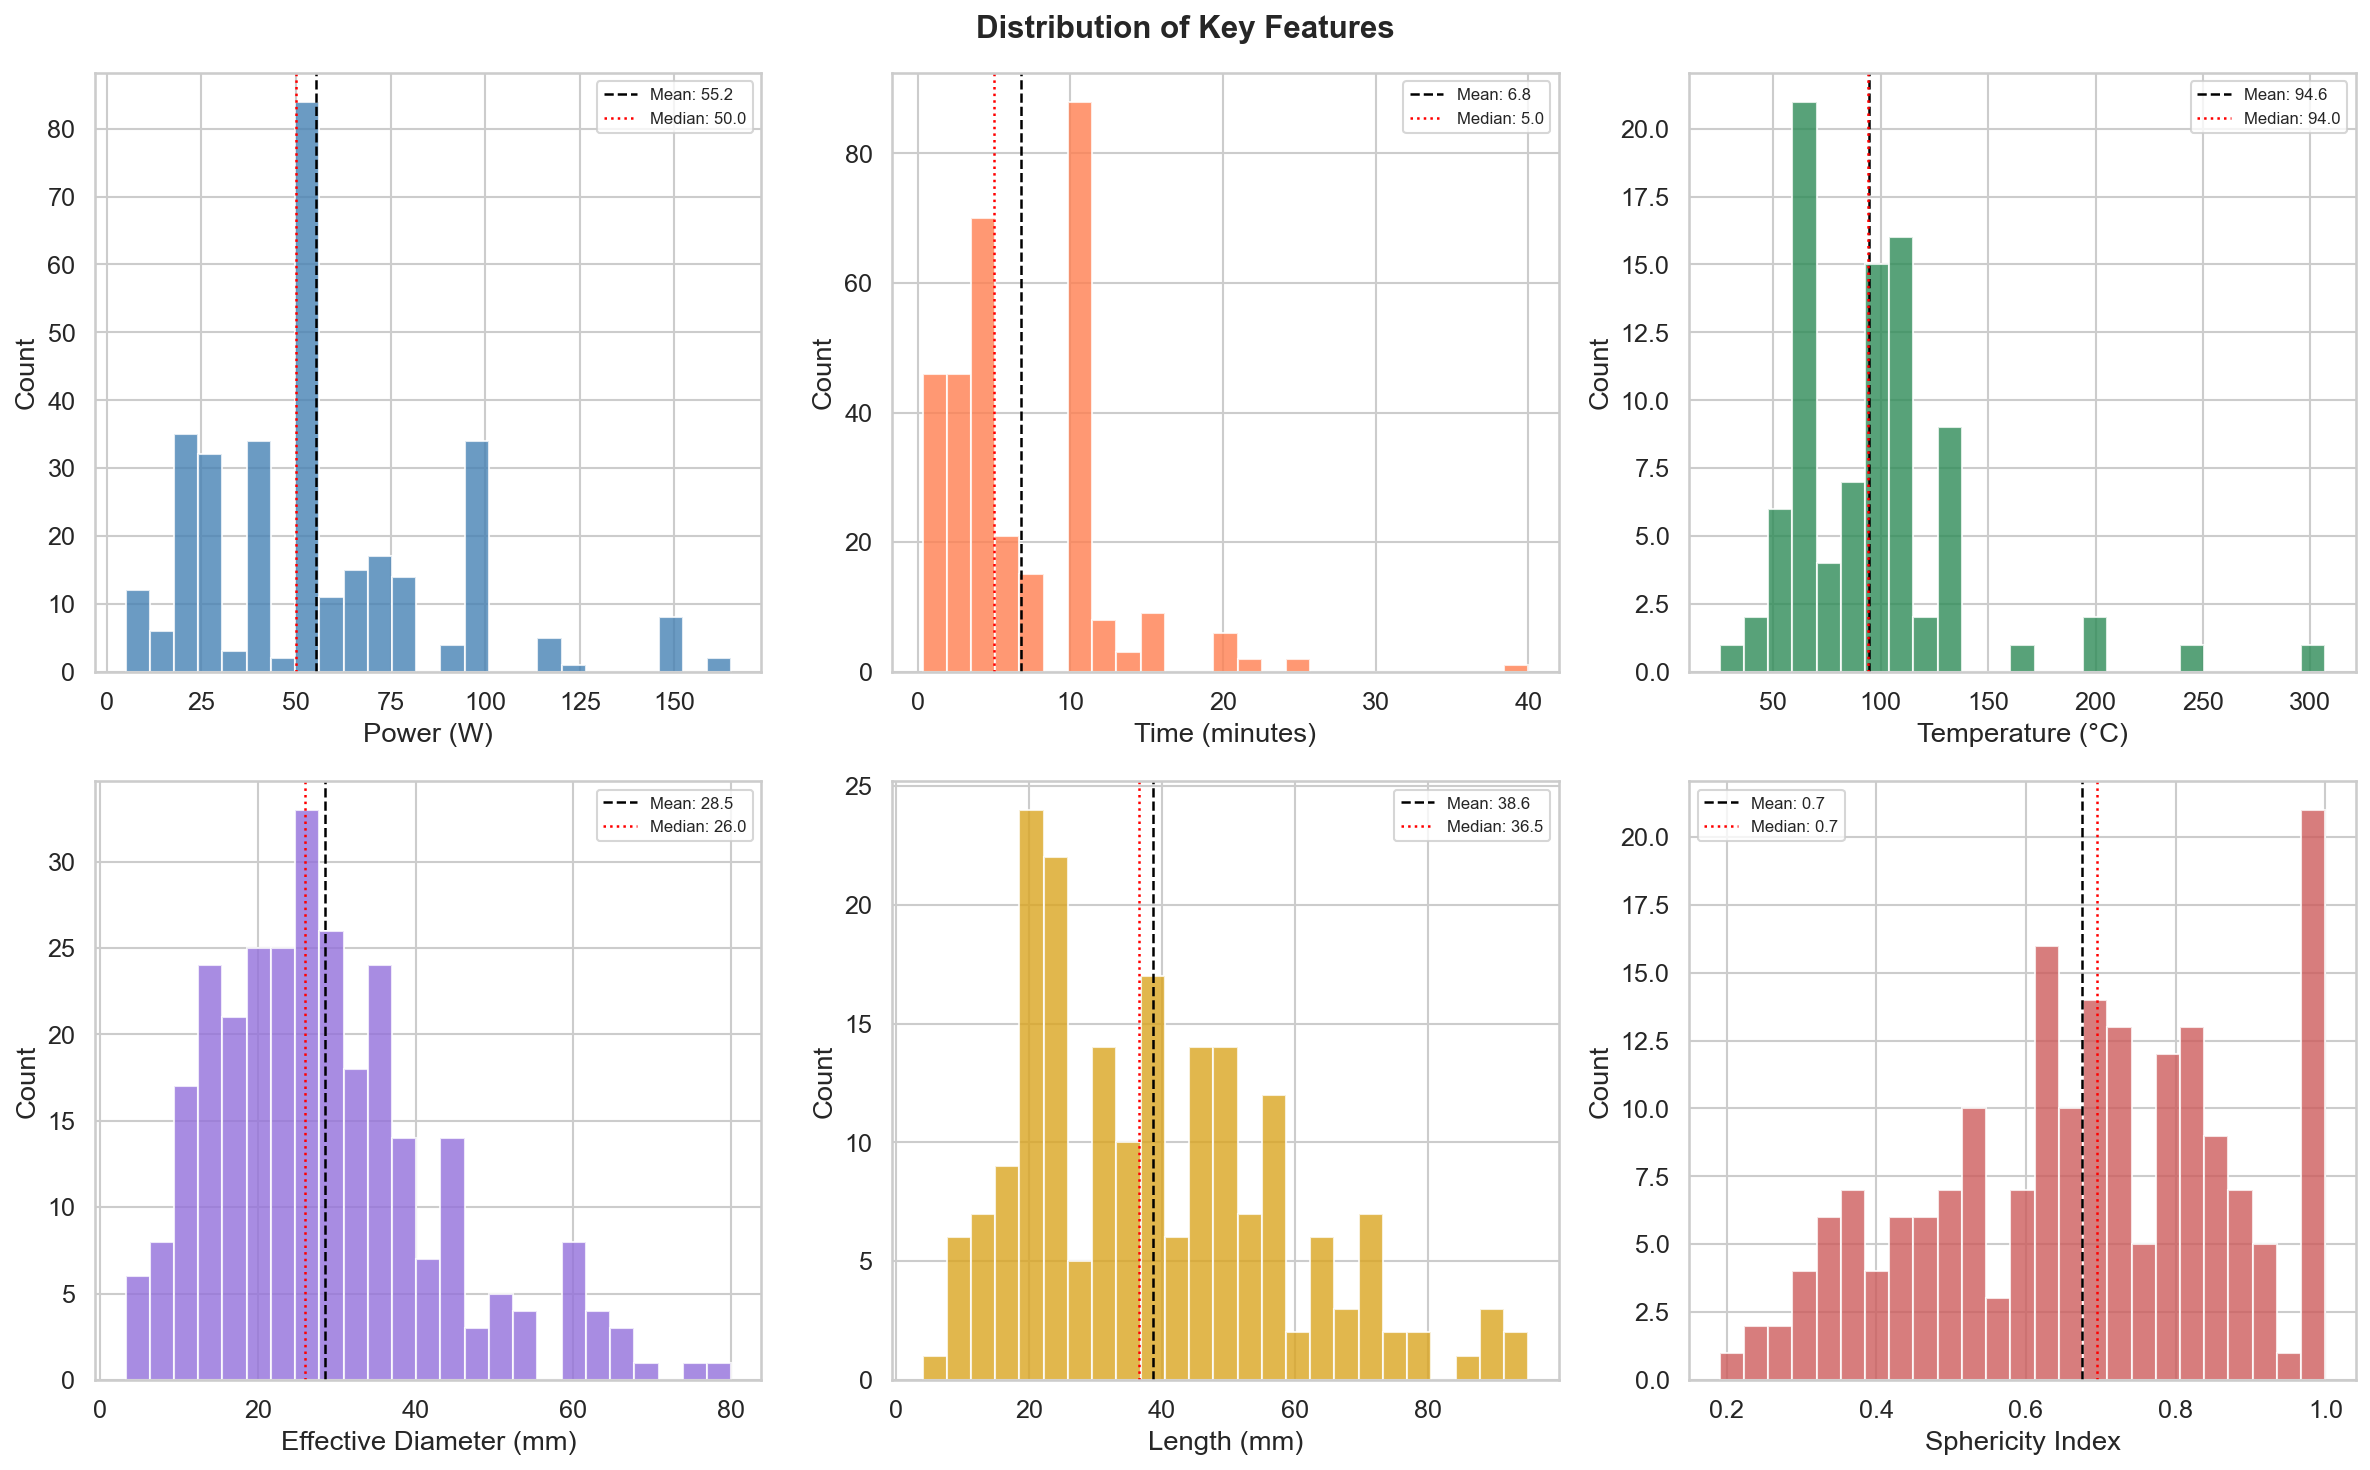
\includegraphics[width=0.95\textwidth]{feature_distributions.png}
\caption{Distribution of key features in the dataset.}
\label{fig:feature-distributions}
\end{figure}

Key observations:
\begin{itemize}
    \item \textbf{Power}: Right-skewed; majority of studies use 20--100\,W, with a mean of $\sim$48\,W (after filtering extreme values).
    \item \textbf{Time}: Most treatments last 1--15 minutes, with 5 and 10 minutes being the most common.
    \item \textbf{Temperature}: Available for only 29.1\% of samples; ranges from 25\,°C to 307\,°C.
    \item \textbf{Effective Diameter}: Approximately normally distributed, mean $\sim$28\,mm.
    \item \textbf{Sphericity Index}: Mean $\sim$0.68, indicating most ablation zones are ellipsoidal.
\end{itemize}

\subsubsection{Correlation Analysis}
\label{sec:correlation}

\begin{figure}[H]
\centering
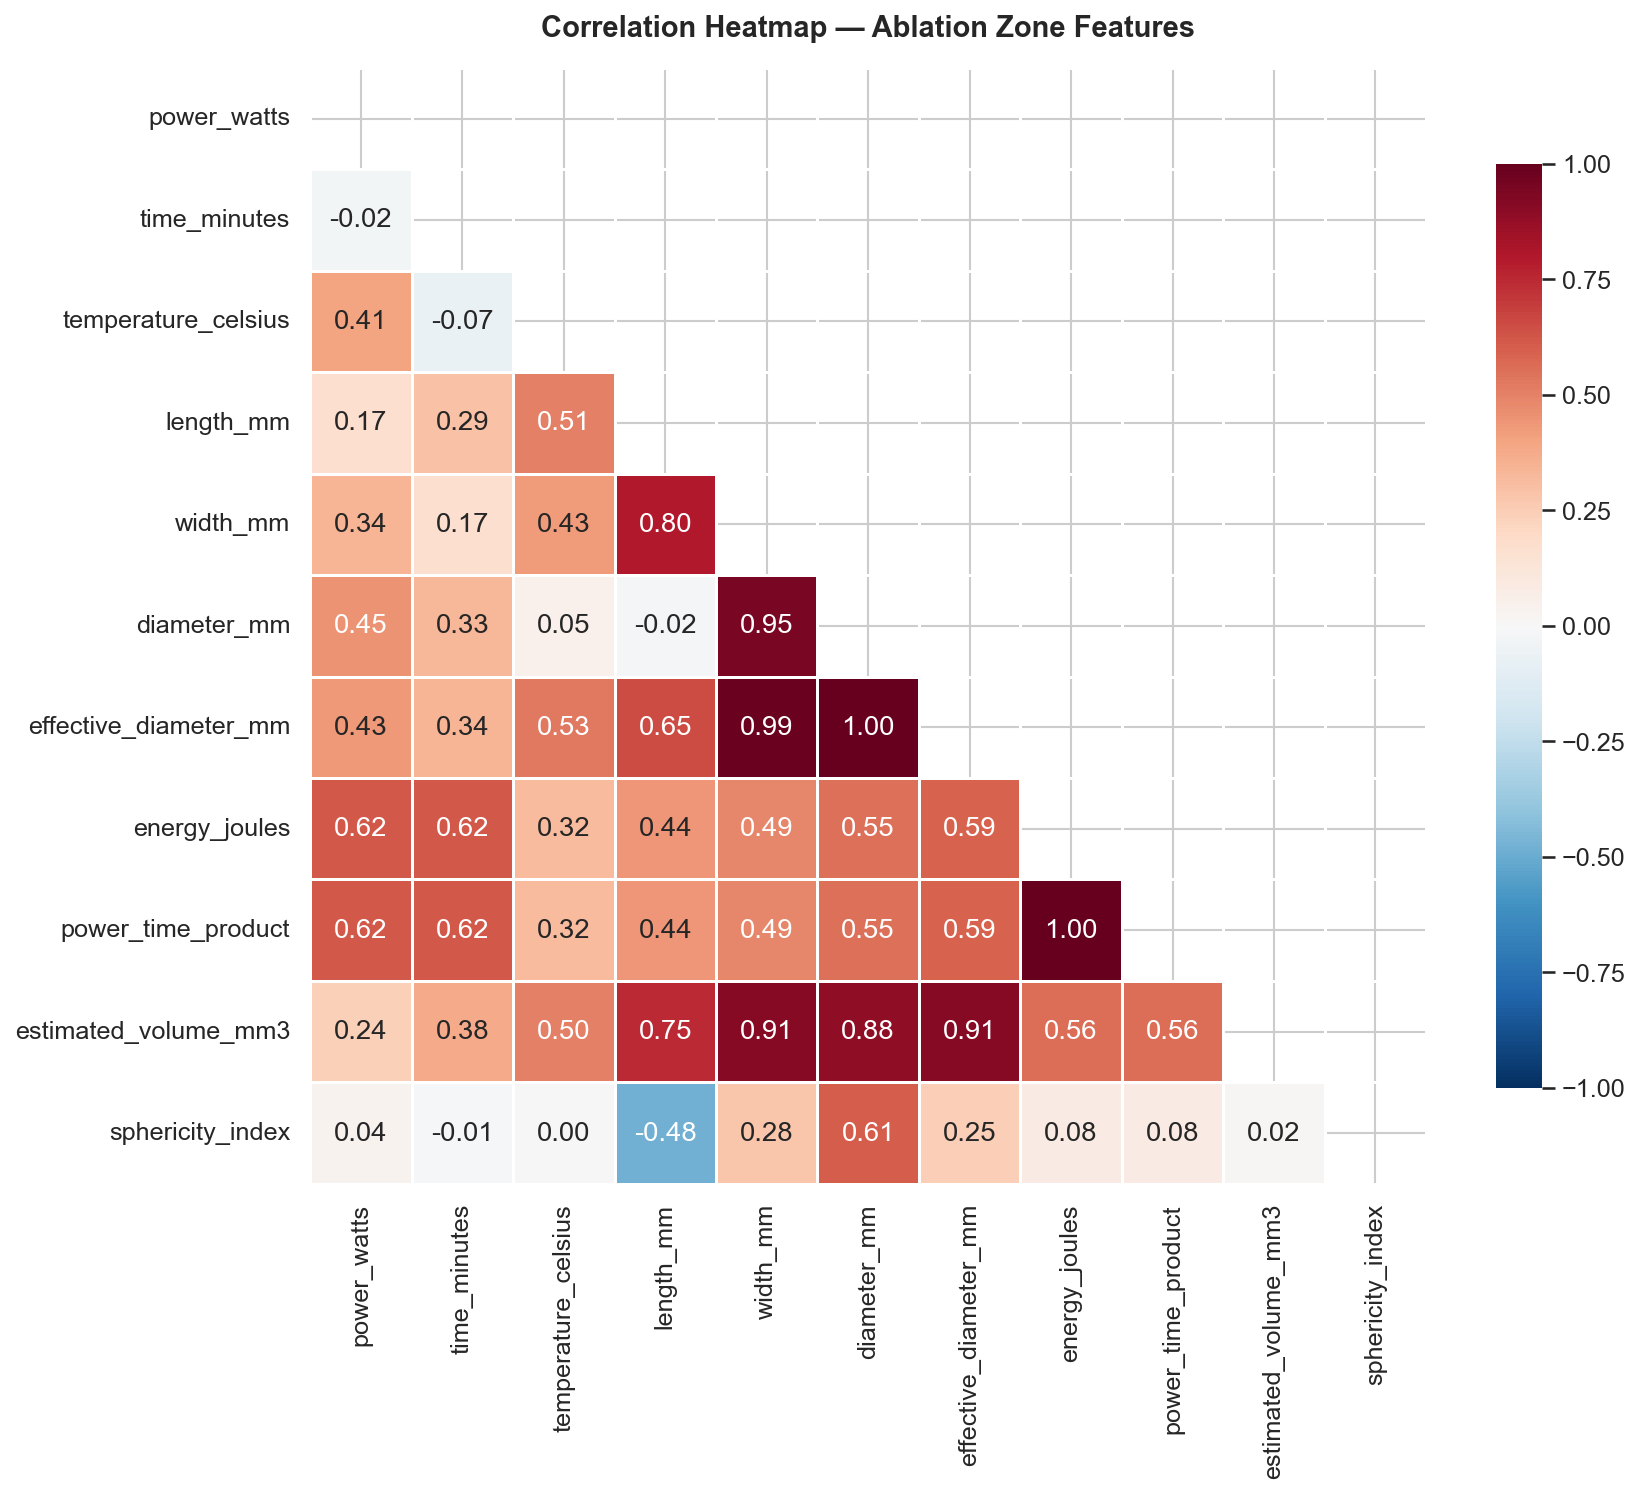
\includegraphics[width=0.85\textwidth]{correlation_heatmap.png}
\caption{Correlation heatmap of numerical features.}
\label{fig:correlation}
\end{figure}

Key correlations with \textbf{effective diameter} (primary target):
\begin{itemize}
    \item \texttt{energy\_joules} (power $\times$ time $\times$ 60): $r = +0.591$ --- strongest input predictor.
    \item \texttt{power\_time\_product}: $r = +0.591$.
    \item \texttt{temperature\_celsius}: $r = +0.531$.
    \item \texttt{power\_watts}: $r = +0.430$.
    \item \texttt{time\_minutes}: $r = +0.343$.
\end{itemize}

The energy delivered (power $\times$ time) is a significantly better predictor than either power or time alone, justifying its inclusion as an engineered feature (Figure~\ref{fig:ablation-vs-inputs}).

\begin{figure}[H]
\centering
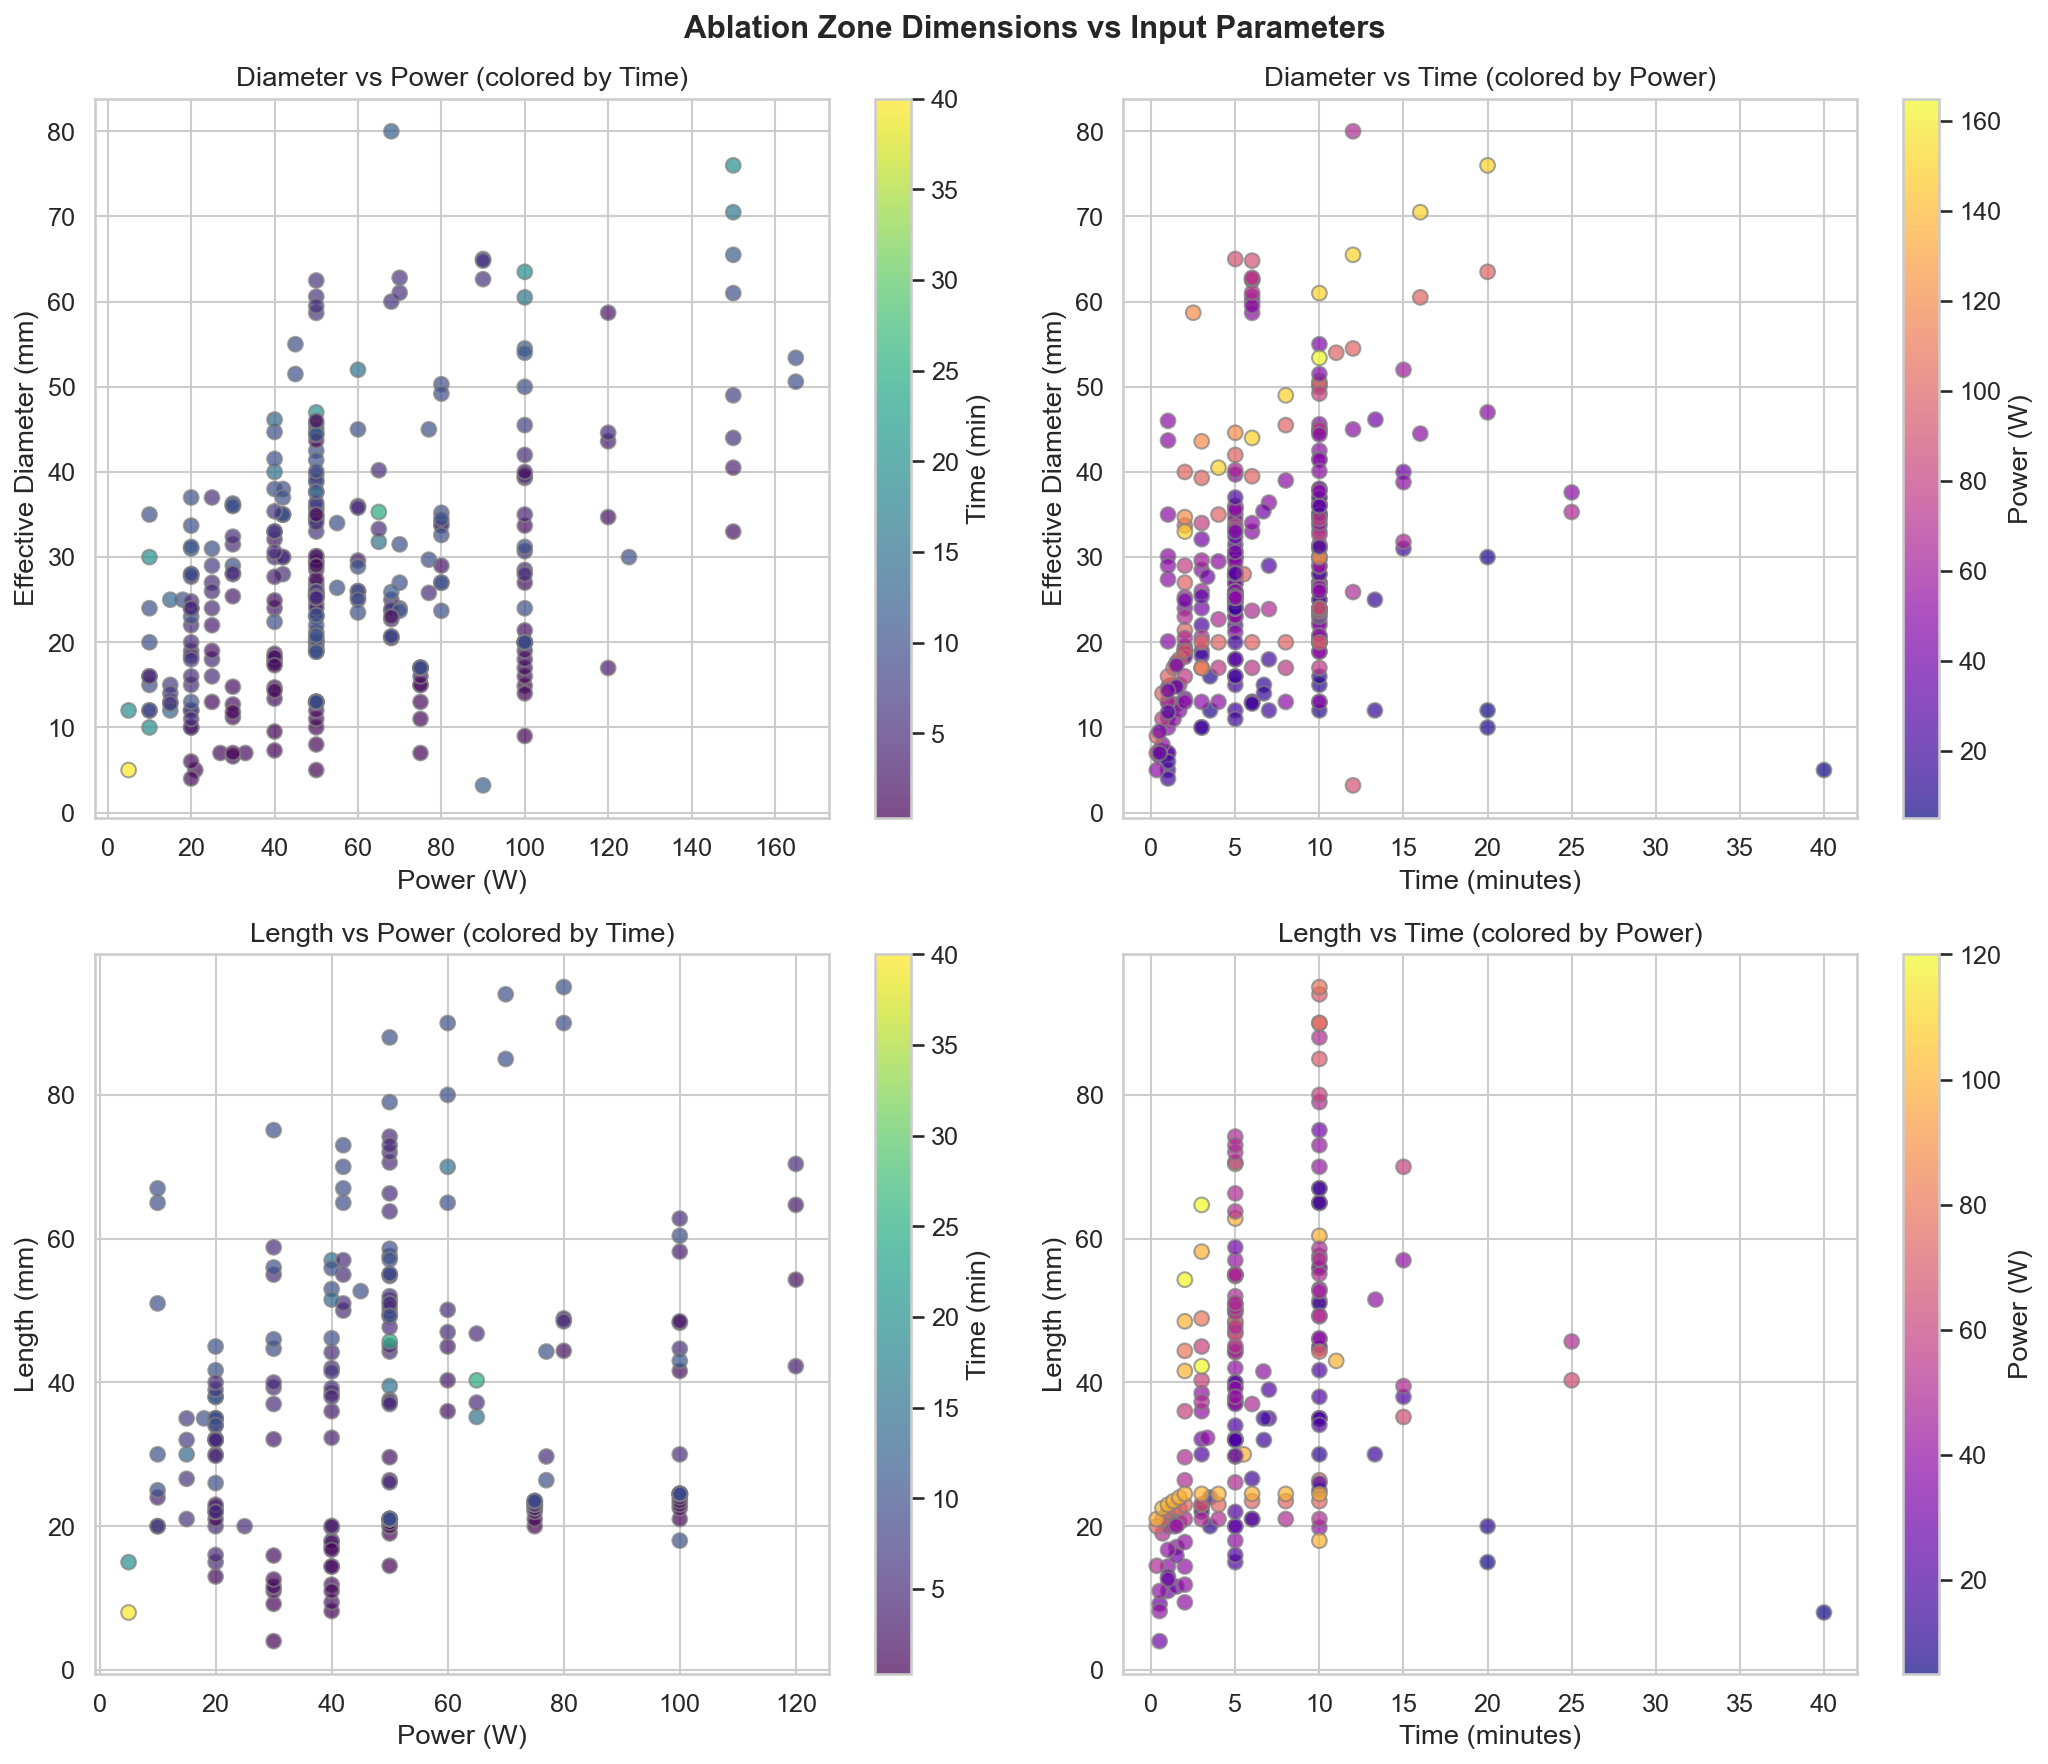
\includegraphics[width=0.95\textwidth]{ablation_vs_inputs.png}
\caption{Ablation zone dimensions vs.\ input parameters.}
\label{fig:ablation-vs-inputs}
\end{figure}

\subsubsection{Missing Value Analysis}
\label{sec:missing-values}

\begin{figure}[H]
\centering
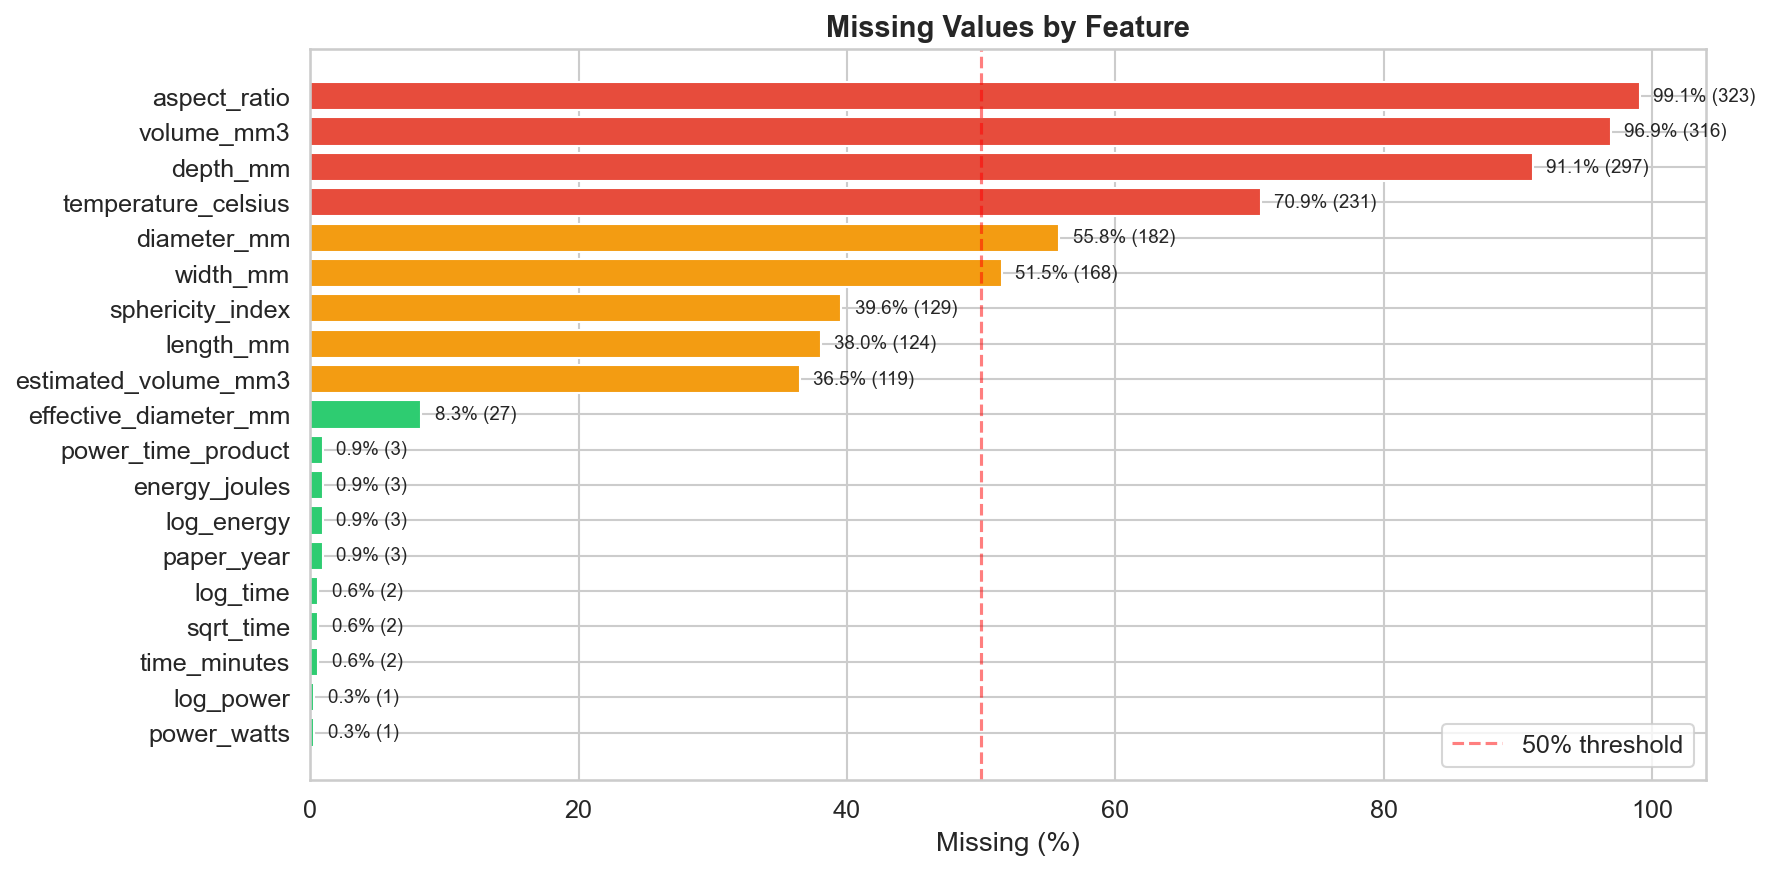
\includegraphics[width=0.85\textwidth]{missing_values.png}
\caption{Missing value percentages by feature.}
\label{fig:missing-values}
\end{figure}

\begin{itemize}
    \item \texttt{aspect\_ratio} (99.1\% missing) and \texttt{volume\_mm3} (96.9\% missing): Too sparse for direct use as targets.
    \item \texttt{temperature\_celsius} (70.9\% missing): Not reliable as an input feature; treated as optional.
    \item \texttt{effective\_diameter\_mm} (8.3\% missing): Primary target, well-populated.
    \item \texttt{length\_mm} (38.0\% missing): Secondary target, moderately populated.
\end{itemize}

\subsubsection{Antenna Type Analysis}
\label{sec:antenna-analysis}

\begin{figure}[H]
\centering
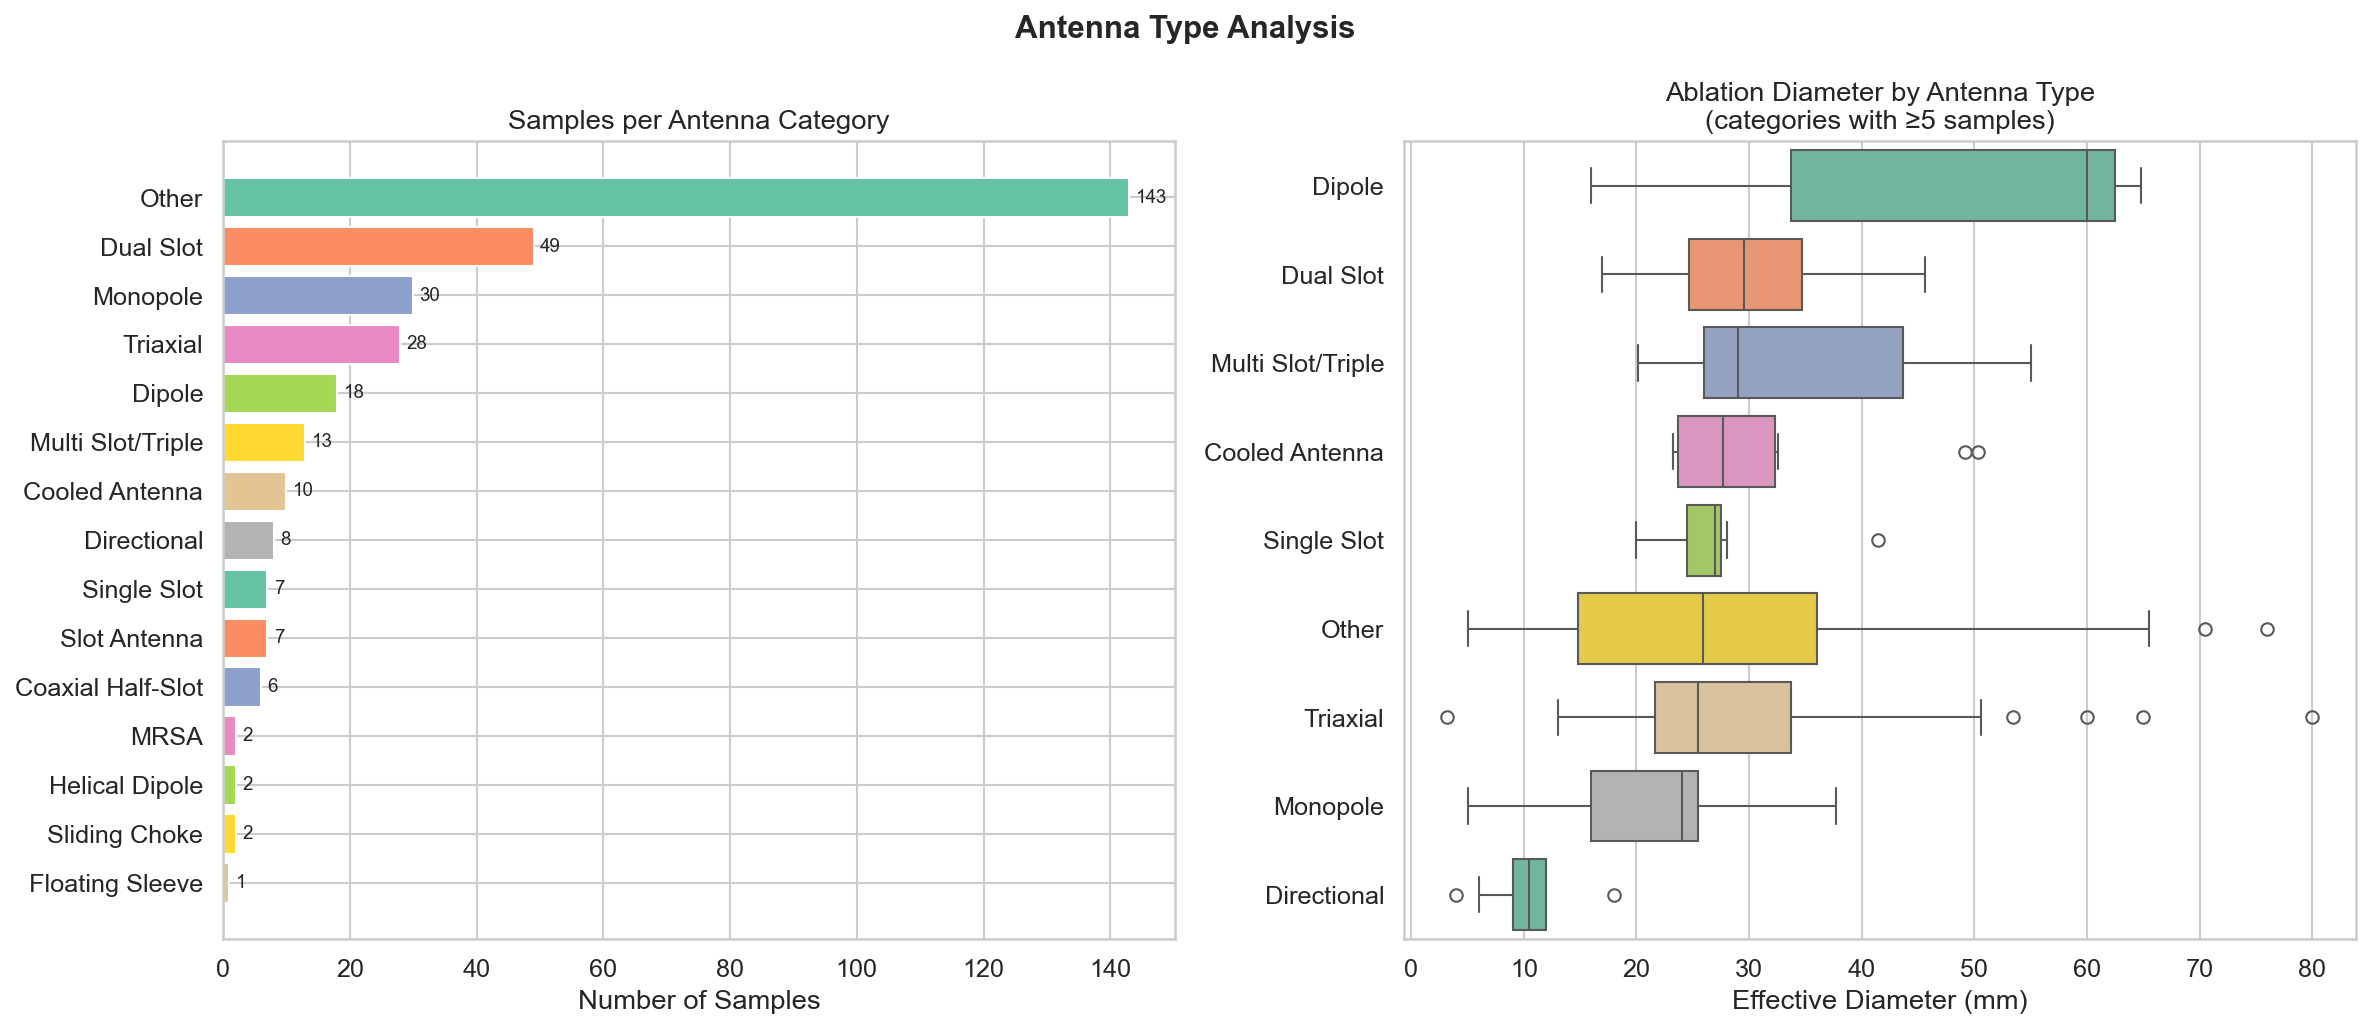
\includegraphics[width=0.85\textwidth]{antenna_distribution.png}
\caption{Distribution of antenna types and their ablation diameters.}
\label{fig:antenna-distribution}
\end{figure}

Fifteen antenna categories were identified. The ``Other'' category (143 samples) includes papers where the antenna type was embedded in the paper title rather than explicitly labelled. The box plot reveals that different antenna types produce significantly different ablation diameters, confirming the importance of antenna type as an input feature.

\subsubsection{Experimental vs.\ Simulated Comparison}
\label{sec:exp-vs-sim}

\begin{figure}[H]
\centering
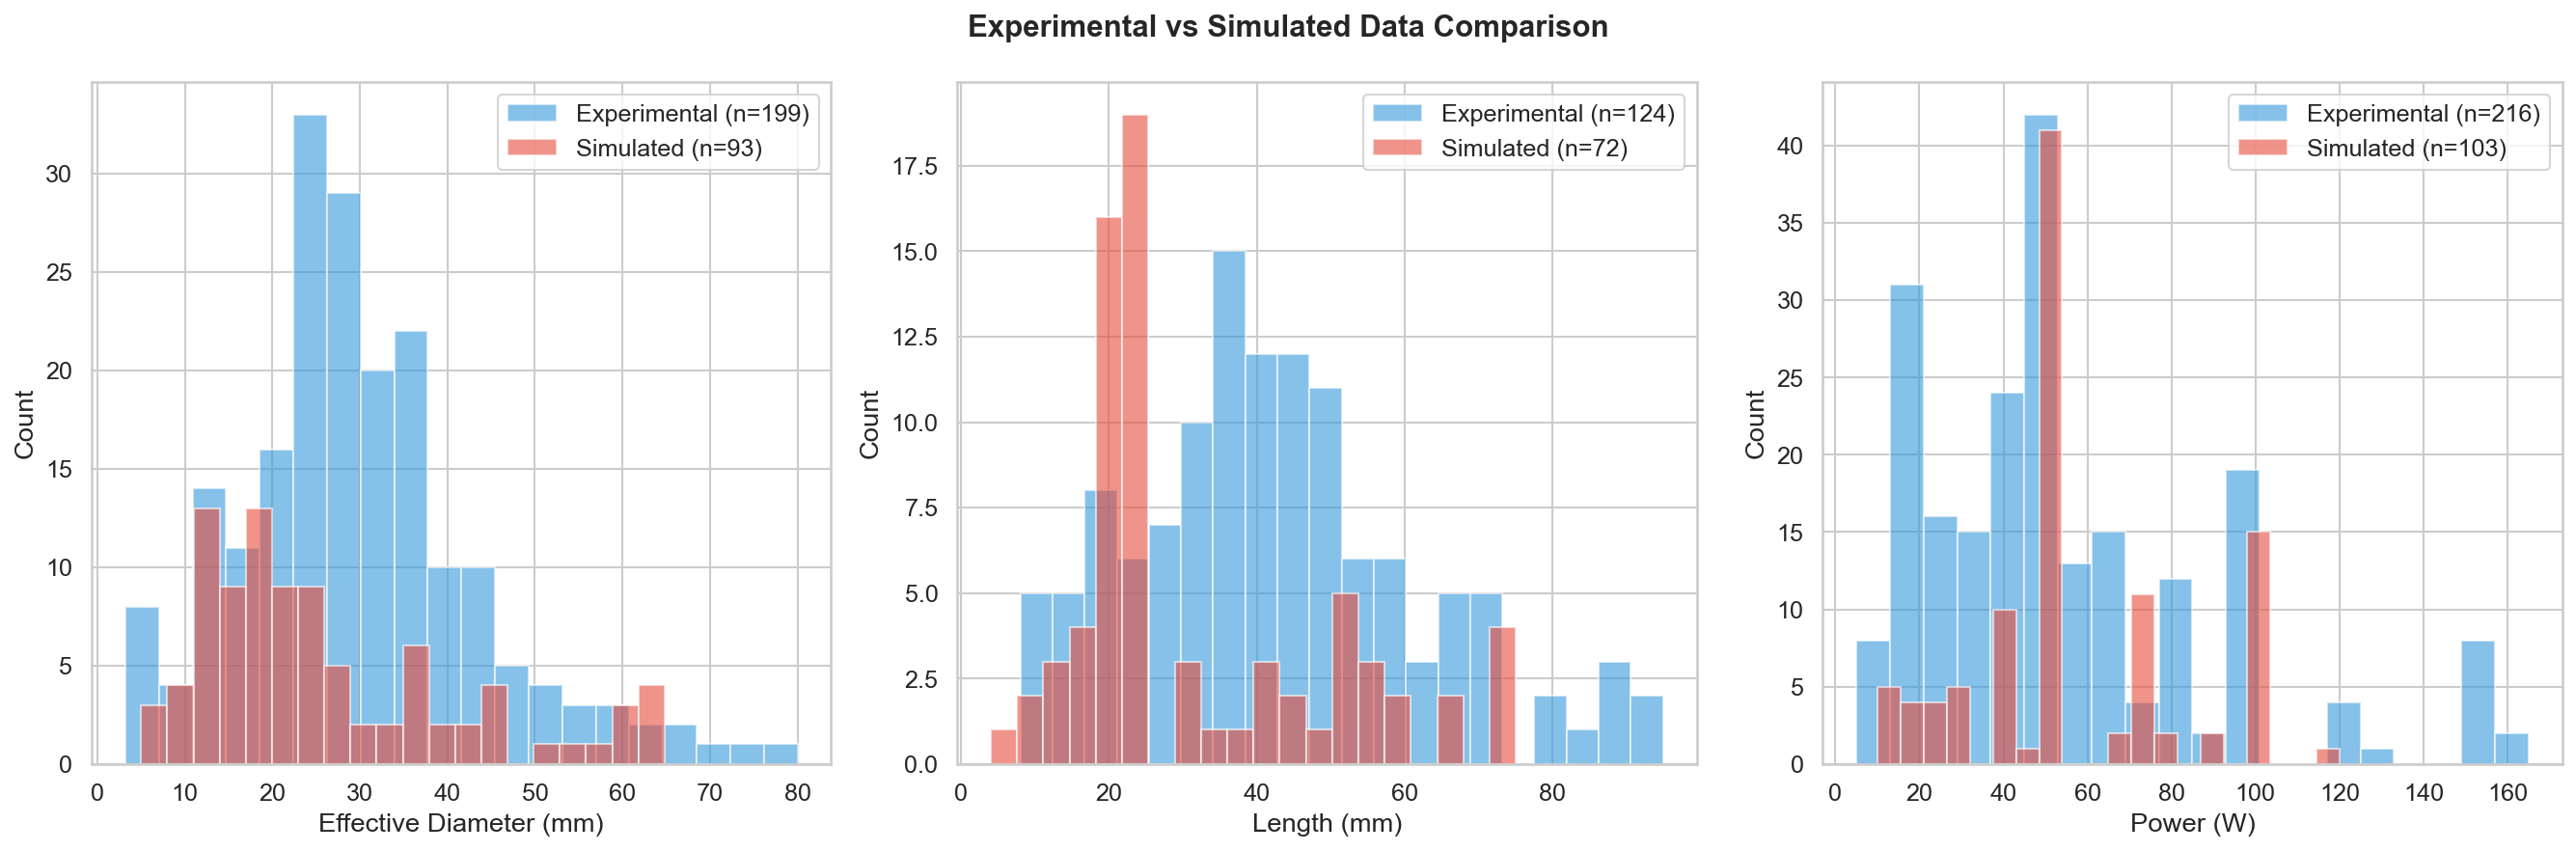
\includegraphics[width=0.85\textwidth]{data_source_comparison.png}
\caption{Comparison of experimental and simulated data distributions.}
\label{fig:data-source-comparison}
\end{figure}

Both datasets show similar distributions for power and ablation dimensions, suggesting they can be combined for training. A binary \texttt{is\_simulated} flag was included as a feature to allow models to account for systematic differences.

% ═════════════════════════════════════════════════════════════
\section{Methodology}
\label{sec:methodology}

\subsection{Data Preprocessing}
\label{sec:preprocessing}

\subsubsection{Feature Engineering}
\label{sec:feature-engineering}

Raw text fields were parsed into numerical features using regex-based extraction. The following features were engineered:

\begin{table}[H]
\centering
\caption{Engineered features and their descriptions.}
\label{tab:features}
\begin{tabular}{@{}ll@{}}
\toprule
\textbf{Feature} & \textbf{Formula / Description} \\
\midrule
\texttt{power\_watts}         & Input power in Watts \\
\texttt{time\_minutes}        & Treatment duration in minutes \\
\texttt{energy\_joules}       & $\text{power} \times \text{time} \times 60$ (total energy delivered) \\
\texttt{power\_time\_product} & $\text{power} \times \text{time}$ \\
\texttt{log\_power}           & $\ln(1 + \text{power})$ \\
\texttt{log\_time}            & $\ln(1 + \text{time})$ \\
\texttt{log\_energy}          & $\ln(1 + \text{energy})$ \\
\texttt{sqrt\_time}           & $\sqrt{\text{time}}$ (models diffusion-like growth) \\
\texttt{is\_simulated}        & 0 = Experimental, 1 = Simulated \\
\texttt{antenna\_encoded}     & Label-encoded antenna category (0--14) \\
\bottomrule
\end{tabular}
\end{table}

\textbf{Rationale for engineered features:}
\begin{itemize}
    \item \textbf{Energy}: Heat generation is proportional to energy deposited, not just power.
    \item \textbf{Log transforms}: Account for diminishing returns at high values (saturation effects).
    \item $\boldsymbol{\sqrt{\text{time}}}$: Thermal diffusion in tissue follows a square-root relationship with time.
    \item \textbf{Interaction term}: Captures the non-linear combined effect of power and time.
\end{itemize}

\subsubsection{Outlier Removal}
\label{sec:outlier-removal}

Samples with power $>200$\,W were removed (7 entries). These were pulsed microwave ablation studies using 25\,kW peak power --- a fundamentally different treatment modality that would distort the model.

\textbf{After outlier removal: 319 samples.}

\subsubsection{Feature Scaling \& Encoding}
\label{sec:scaling}

\begin{itemize}
    \item \textbf{StandardScaler} ($z$-score normalization) was applied for SVR, KNN, and MLP models (fitted on training data only to prevent data leakage).
    \item \textbf{Tree-based models} (Random Forest, Gradient Boosting) do not require scaling.
    \item \textbf{LabelEncoder} was used for the 15 antenna categories.
\end{itemize}

\subsubsection{Train--Test Split}
\label{sec:train-test-split}

An 80/20 random split (with \texttt{random\_state=42} for reproducibility) was used:

\begin{table}[H]
\centering
\caption{Train--test split sizes for each target variable.}
\label{tab:split}
\begin{tabular}{@{}lcc@{}}
\toprule
\textbf{Target} & \textbf{Train Samples} & \textbf{Test Samples} \\
\midrule
Effective Diameter & 233 & 59 \\
Length             & 156 & 40 \\
Both (multi-output)& 152 & 39 \\
\bottomrule
\end{tabular}
\end{table}

\subsection{Machine Learning Models}
\label{sec:ml-models}

Six regression models were selected to cover a range of algorithmic approaches:

\subsubsection{Ridge Regression}
\label{sec:ridge}

A linear regression model with \textbf{L2 regularization} (penalty on the sum of squared coefficients). It serves as the baseline linear model. Ridge is suitable for preventing multicollinearity issues arising from the correlated features (e.g., \texttt{power\_watts} and \texttt{energy\_joules}).

\begin{itemize}
    \item \textbf{Hyperparameters tuned}: $\alpha \in \{0.01,\; 0.1,\; 1.0,\; 10.0,\; 100.0\}$
\end{itemize}

\subsubsection{K-Nearest Neighbors (KNN)}
\label{sec:knn}

A non-parametric, instance-based method that predicts by averaging the target values of the $k$ most similar training samples. KNN captures local patterns without making assumptions about the data distribution.

\begin{itemize}
    \item \textbf{Hyperparameters tuned}: $k \in \{3, 5, 7, 9, 11\}$, weights $\in$ \{uniform, distance\}, metric $\in$ \{euclidean, manhattan\}
\end{itemize}

\subsubsection{Support Vector Regression (SVR)}
\label{sec:svr}

SVR maps input features to a higher-dimensional space using a \textbf{Radial Basis Function (RBF) kernel} and finds a hyperplane that fits the data within an $\varepsilon$-insensitive tube. It is effective for small datasets and can model non-linear relationships.

\begin{itemize}
    \item \textbf{Hyperparameters tuned}: $C \in \{0.1, 1.0, 10.0, 100.0\}$, $\gamma \in \{\text{scale}, \text{auto}, 0.01, 0.1\}$, $\varepsilon \in \{0.01, 0.1, 0.5\}$
\end{itemize}

\subsubsection{Random Forest}
\label{sec:random-forest}

An \textbf{ensemble of decision trees}, each trained on a random bootstrap sample of the data with random feature subsets. The final prediction is the average of all trees. Random Forest is robust, handles non-linearity well, and provides feature importance rankings.

\begin{itemize}
    \item \textbf{Hyperparameters tuned}: \texttt{n\_estimators} $\in \{50, 100, 200\}$, \texttt{max\_depth} $\in \{5, 10, 15, \text{None}\}$, \texttt{min\_samples\_split} $\in \{2, 5\}$, \texttt{min\_samples\_leaf} $\in \{1, 2\}$
\end{itemize}

\subsubsection{Gradient Boosting Regressor}
\label{sec:gradient-boosting}

Builds an \textbf{additive ensemble of decision trees} sequentially, where each new tree corrects the errors of the previous ensemble. This iterative approach typically achieves higher accuracy than Random Forest at the cost of higher overfitting risk.

\begin{itemize}
    \item \textbf{Hyperparameters tuned}: \texttt{n\_estimators} $\in \{50, 100, 200\}$, \texttt{max\_depth} $\in \{3, 5, 7\}$, \texttt{learning\_rate} $\in \{0.01, 0.05, 0.1, 0.2\}$, \texttt{subsample} $\in \{0.8, 1.0\}$
\end{itemize}

\subsubsection{Multi-Layer Perceptron (MLP)}
\label{sec:mlp}

A feedforward \textbf{artificial neural network} with one or two hidden layers, trained using backpropagation. MLP can approximate complex non-linear mappings but requires careful regularization to avoid overfitting on small datasets.

\begin{itemize}
    \item \textbf{Hyperparameters tuned}: \texttt{hidden\_layer\_sizes} $\in \{(50,),\; (100,),\; (50, 25),\; (100, 50)\}$, activation $\in$ \{relu, tanh\}, $\alpha \in \{0.001, 0.01, 0.1\}$, learning\_rate = adaptive
\end{itemize}

\subsection{Evaluation Metrics}
\label{sec:metrics}

Four metrics were used for comprehensive model evaluation:

\begin{table}[H]
\centering
\caption{Evaluation metrics used for model comparison.}
\label{tab:metrics}
\begin{tabular}{@{}lll@{}}
\toprule
\textbf{Metric} & \textbf{Formula} & \textbf{Interpretation} \\
\midrule
$R^2$ Score & $1 - \dfrac{SS_{\text{res}}}{SS_{\text{tot}}}$ & Proportion of variance explained ($1.0$ = perfect) \\[1em]
MAE & $\dfrac{1}{n}\displaystyle\sum_{i=1}^{n}|y_i - \hat{y}_i|$ & Average absolute prediction error (mm) \\[1em]
RMSE & $\sqrt{\dfrac{1}{n}\displaystyle\sum_{i=1}^{n}(y_i - \hat{y}_i)^2}$ & Penalizes larger errors more heavily \\[1em]
MAPE & $\dfrac{100}{n}\displaystyle\sum_{i=1}^{n}\dfrac{|y_i - \hat{y}_i|}{|y_i|}$ & Relative error as a percentage \\
\bottomrule
\end{tabular}
\end{table}

\subsection{Hyperparameter Tuning}
\label{sec:tuning}

\textbf{GridSearchCV} with \textbf{10-fold cross-validation} was used for hyperparameter optimization. For each model:

\begin{enumerate}
    \item All combinations of hyperparameters were evaluated.
    \item The combination maximizing cross-validated $R^2$ was selected.
    \item The model was retrained on the full training set with the best parameters.
    \item Final evaluation was performed on the held-out test set.
\end{enumerate}

This approach ensures that model selection is robust and not overly optimized to a single train--test split.

% ═════════════════════════════════════════════════════════════
\section{Results \& Discussion}
\label{sec:results}

\subsection{Effective Diameter Prediction}
\label{sec:diameter-results}

\begin{table}[H]
\centering
\caption{Model comparison for effective diameter prediction. Best values in \textbf{bold}.}
\label{tab:diameter-results}
\resizebox{\textwidth}{!}{%
\begin{tabular}{@{}lcccccp{5cm}@{}}
\toprule
\textbf{Model} & \textbf{CV $R^2$} & \textbf{Test $R^2$} & \textbf{MAE (mm)} & \textbf{RMSE (mm)} & \textbf{MAPE (\%)} & \textbf{Best Hyperparameters} \\
\midrule
\textbf{Random Forest} $\star$ & 0.5293 & \textbf{0.6952} & \textbf{6.02} & \textbf{7.70} & \textbf{26.7} & n\_est=200, max\_depth=5, min\_samples\_leaf=2 \\
Gradient Boosting    & 0.5047 & 0.6789 & 6.23 & 7.90 & 28.7 & lr=0.01, max\_depth=5, n\_est=200 \\
Ridge Regression     & 0.3542 & 0.5313 & 7.90 & 9.55 & 39.3 & $\alpha$=10.0 \\
KNN                  & 0.4804 & 0.5255 & 7.74 & 9.60 & 34.3 & $k$=7, metric=manhattan, weights=uniform \\
SVR                  & 0.4262 & 0.5138 & 6.91 & 9.72 & 27.8 & $C$=100, $\gamma$=auto, $\varepsilon$=0.5 \\
MLP Neural Network   & 0.4542 & $-$0.0102 & 11.59 & 14.01 & 54.2 & hidden=(50,25), act=relu \\
\bottomrule
\end{tabular}%
}
\end{table}

\begin{figure}[H]
\centering
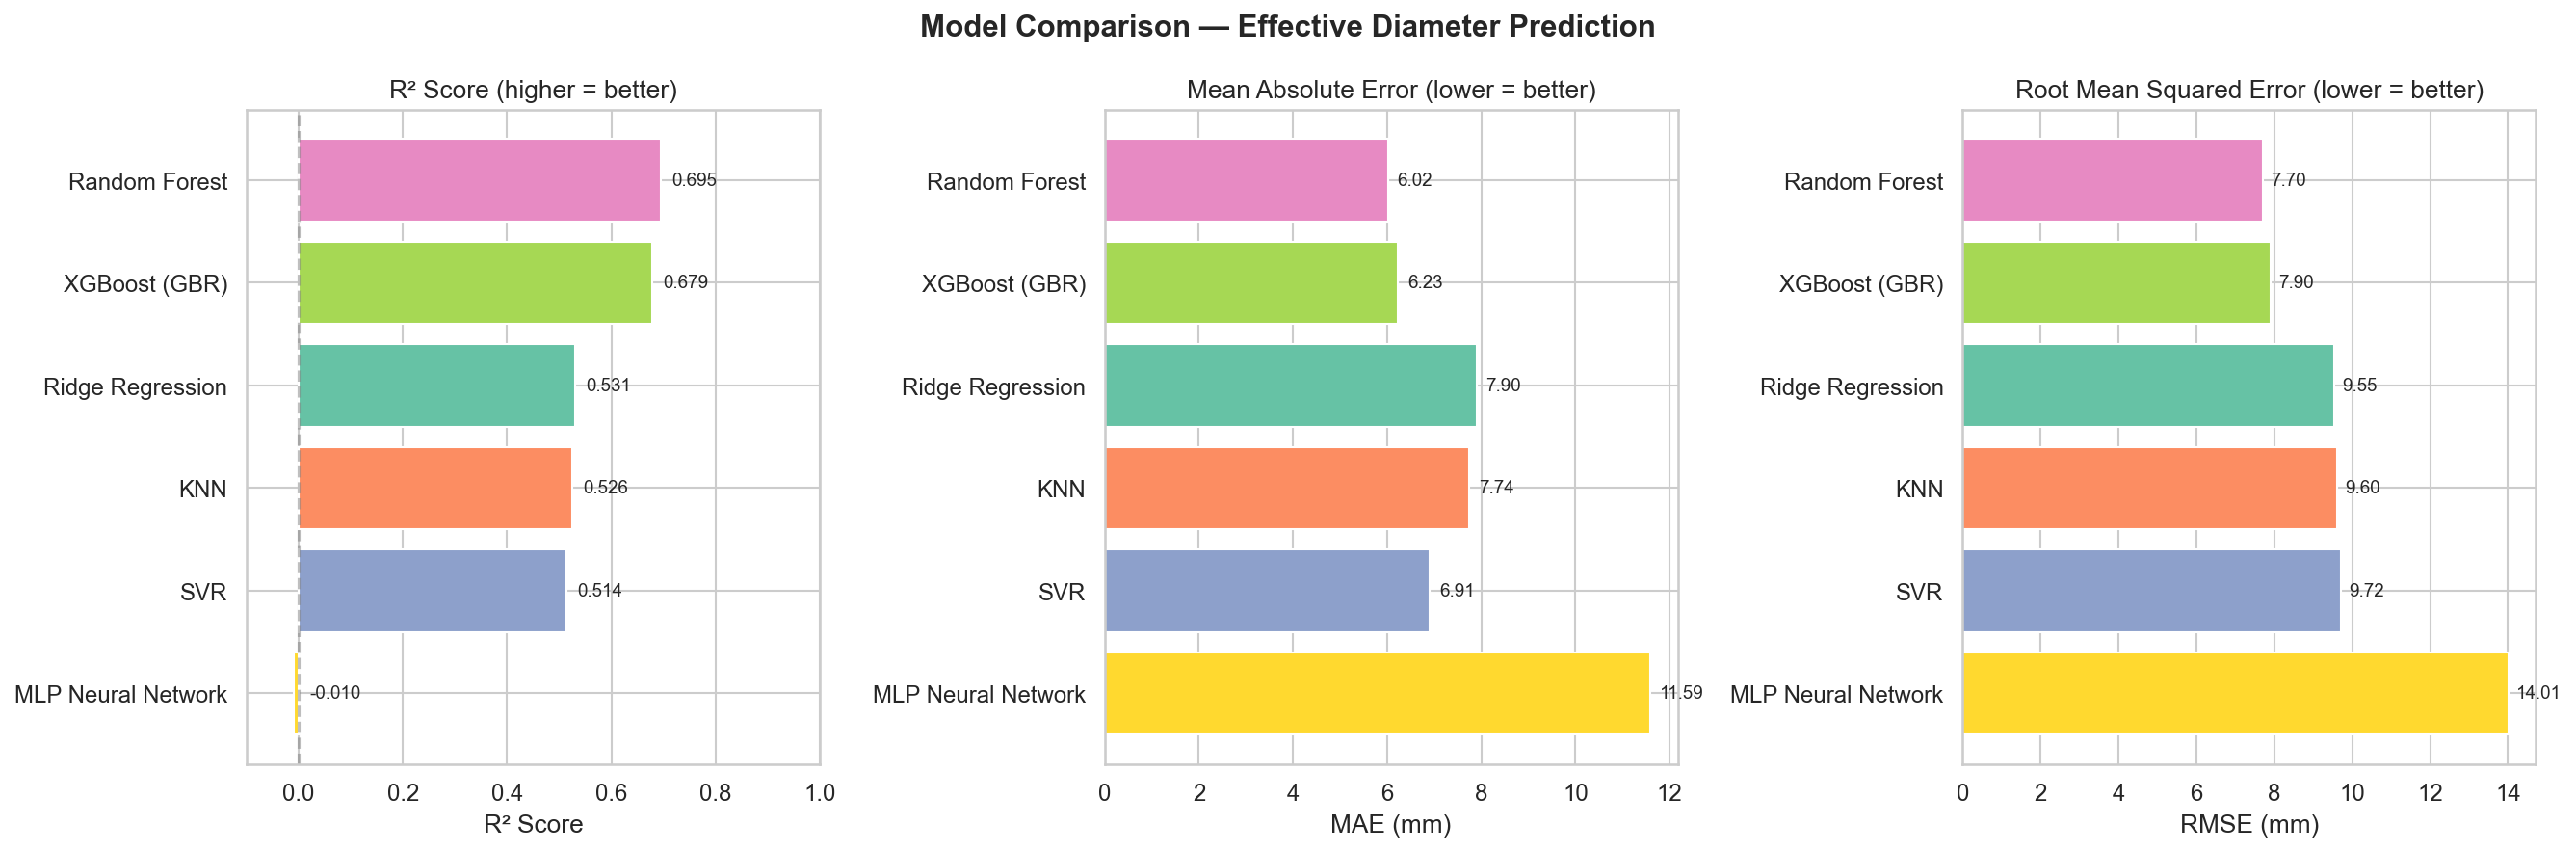
\includegraphics[width=0.85\textwidth]{model_comparison_diameter.png}
\caption{Model comparison for effective diameter prediction.}
\label{fig:model-comparison-diameter}
\end{figure}

\textbf{Random Forest} achieved the best performance with $R^2 = 0.695$ and MAE $= 6.02$\,mm, meaning the model explains $\sim$70\% of the variance in ablation diameter with an average prediction error of only 6\,mm.

\subsection{Length Prediction}
\label{sec:length-results}

\begin{table}[H]
\centering
\caption{Model comparison for length prediction. Best values in \textbf{bold}.}
\label{tab:length-results}
\resizebox{\textwidth}{!}{%
\begin{tabular}{@{}lcccccp{5.5cm}@{}}
\toprule
\textbf{Model} & \textbf{CV $R^2$} & \textbf{Test $R^2$} & \textbf{MAE (mm)} & \textbf{RMSE (mm)} & \textbf{MAPE (\%)} & \textbf{Best Hyperparameters} \\
\midrule
\textbf{Gradient Boosting} $\star$ & 0.6690 & \textbf{0.5118} & 10.93 & \textbf{13.76} & 36.8 & lr=0.01, max\_depth=7, n\_est=200 \\
Random Forest        & 0.6420 & 0.5032 & 10.67 & 13.88 & 35.5 & max\_depth=15, n\_est=200 \\
MLP Neural Network   & 0.5119 & 0.4875 & \textbf{9.97} & 14.10 & \textbf{29.5} & hidden=(100,), act=tanh \\
SVR                  & 0.6180 & 0.3445 & 10.74 & 15.95 & 36.8 & $C$=100, $\gamma$=auto, $\varepsilon$=0.01 \\
KNN                  & 0.6008 & 0.2954 & 11.33 & 16.53 & 36.1 & $k$=3, metric=manhattan, weights=distance \\
Ridge Regression     & 0.3994 & 0.2580 & 12.50 & 16.97 & 44.4 & $\alpha$=0.1 \\
\bottomrule
\end{tabular}%
}
\end{table}

\begin{figure}[H]
\centering
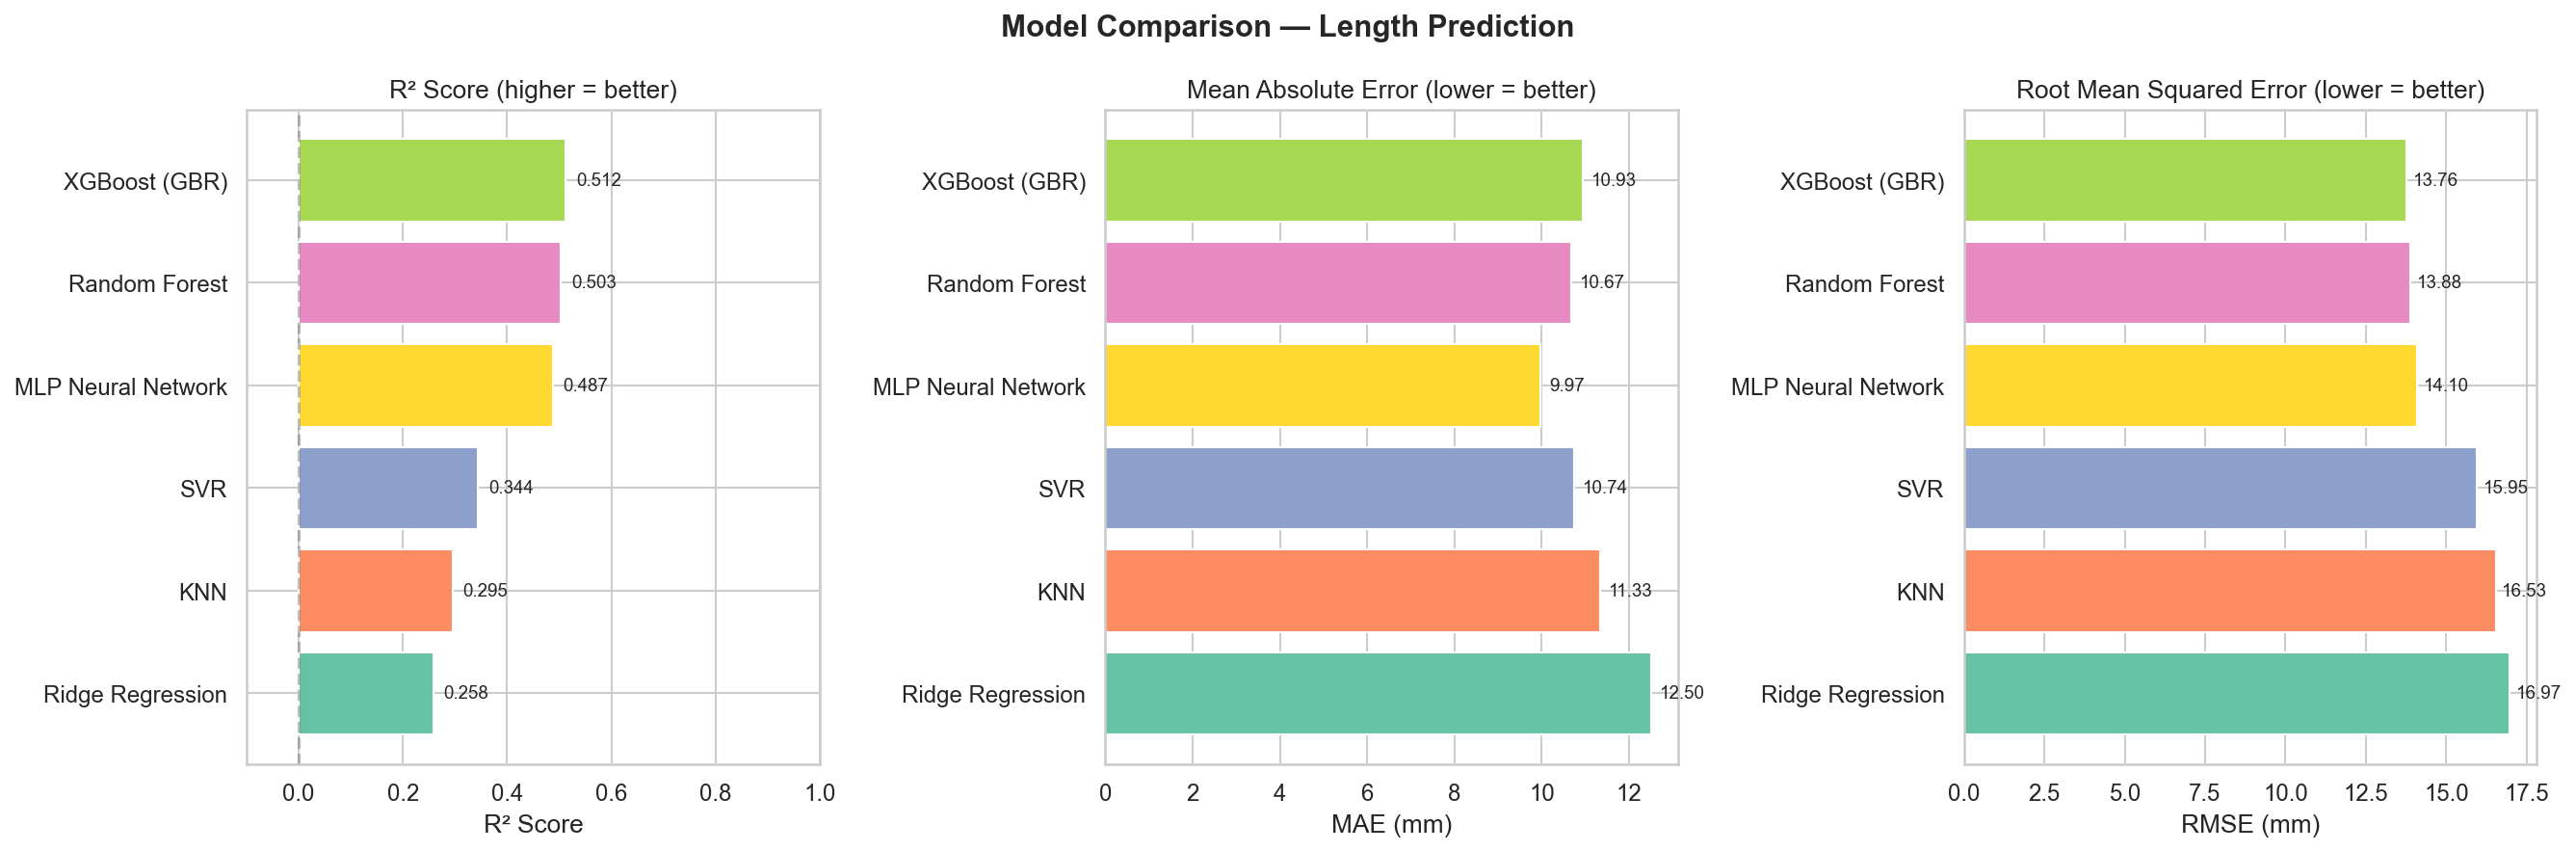
\includegraphics[width=0.85\textwidth]{model_comparison_length.png}
\caption{Model comparison for length prediction.}
\label{fig:model-comparison-length}
\end{figure}

Length prediction is more challenging (lower $R^2$ values), likely because the longitudinal extent of the ablation zone is more sensitive to antenna-specific parameters not captured in our feature set (e.g., antenna length, slot positions, dielectric properties).

\subsection{Best Model Analysis}
\label{sec:best-model}

\subsubsection{Predicted vs.\ Actual}
\label{sec:pred-vs-actual}

\begin{figure}[H]
\centering
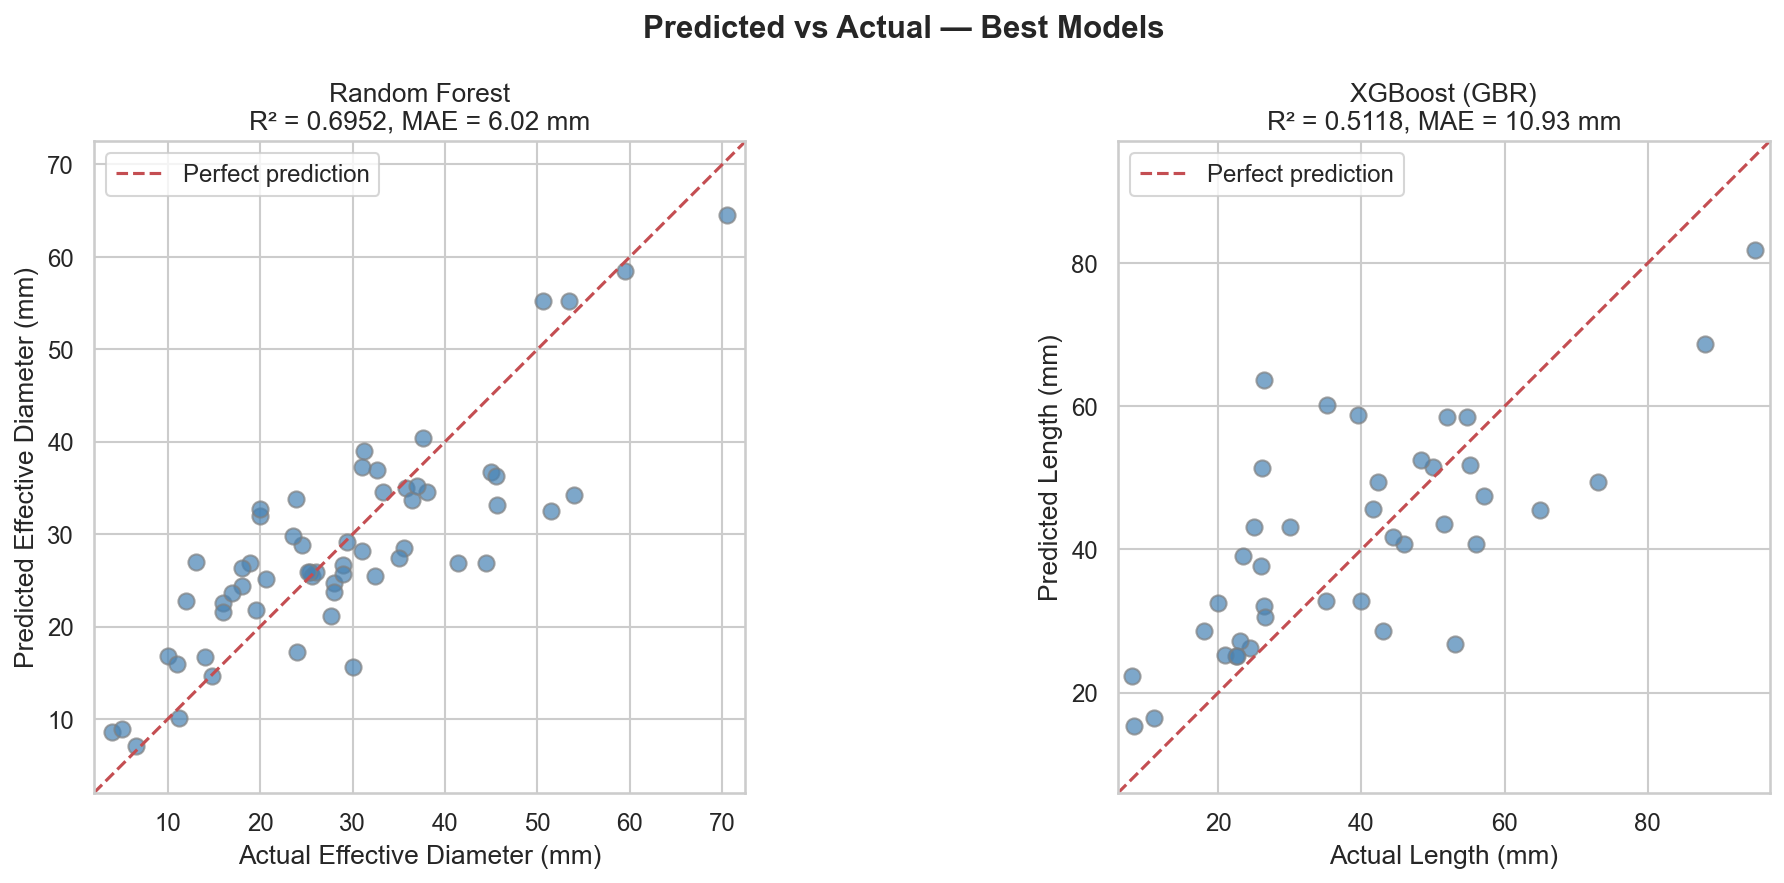
\includegraphics[width=0.85\textwidth]{predicted_vs_actual.png}
\caption{Predicted vs.\ actual values for the best models.}
\label{fig:pred-vs-actual}
\end{figure}

The predicted vs.\ actual plots show that:
\begin{itemize}
    \item \textbf{Diameter}: Points cluster tightly around the 45° line for the 15--45\,mm range, with some scatter at extremes.
    \item \textbf{Length}: More variance, particularly for longer ablation zones ($>50$\,mm).
\end{itemize}

\subsubsection{Residual Analysis}
\label{sec:residual}

\begin{figure}[H]
\centering
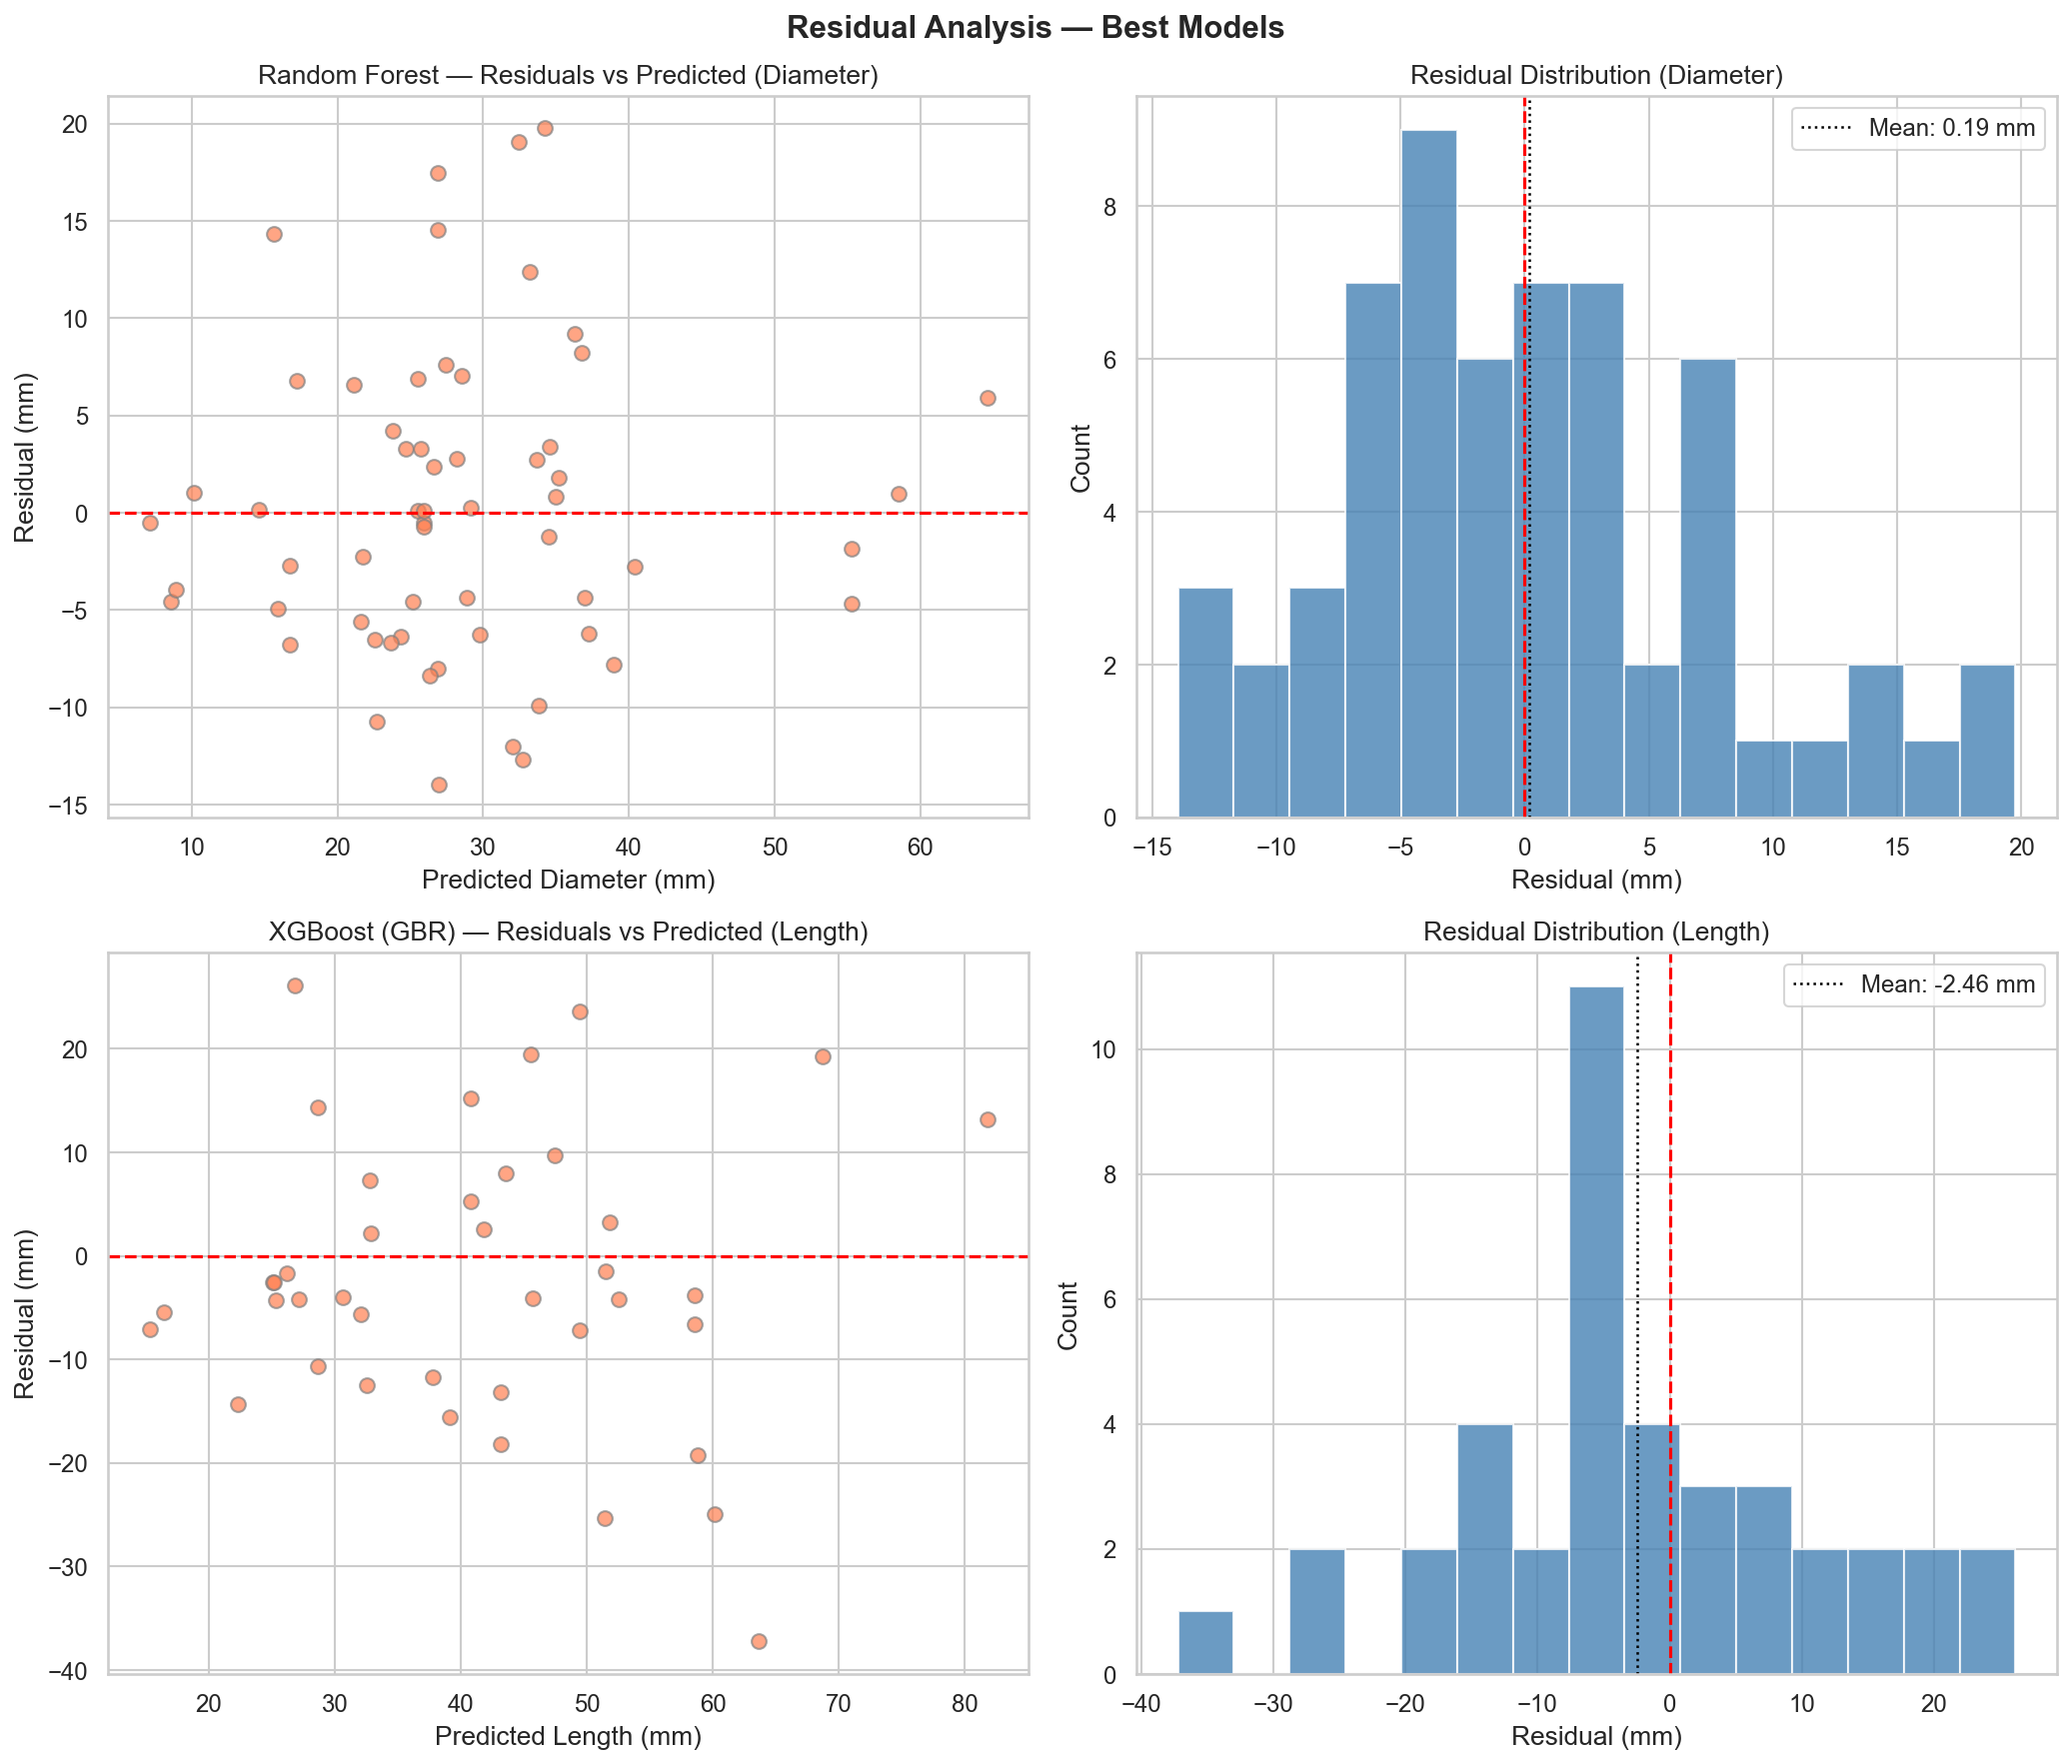
\includegraphics[width=0.95\textwidth]{residual_analysis.png}
\caption{Residual analysis for the best models (residuals vs.\ predicted values and residual distributions).}
\label{fig:residual-analysis}
\end{figure}

The residual plots reveal:
\begin{itemize}
    \item \textbf{No systematic bias}: Residuals are approximately centred around zero.
    \item \textbf{Residual distribution}: Roughly normal, supporting the validity of our regression analysis.
    \item \textbf{Slight heteroscedasticity}: Variance increases for larger predicted values (expected in physical systems).
\end{itemize}

\subsubsection{Feature Importance}
\label{sec:feature-importance}

\begin{figure}[H]
\centering
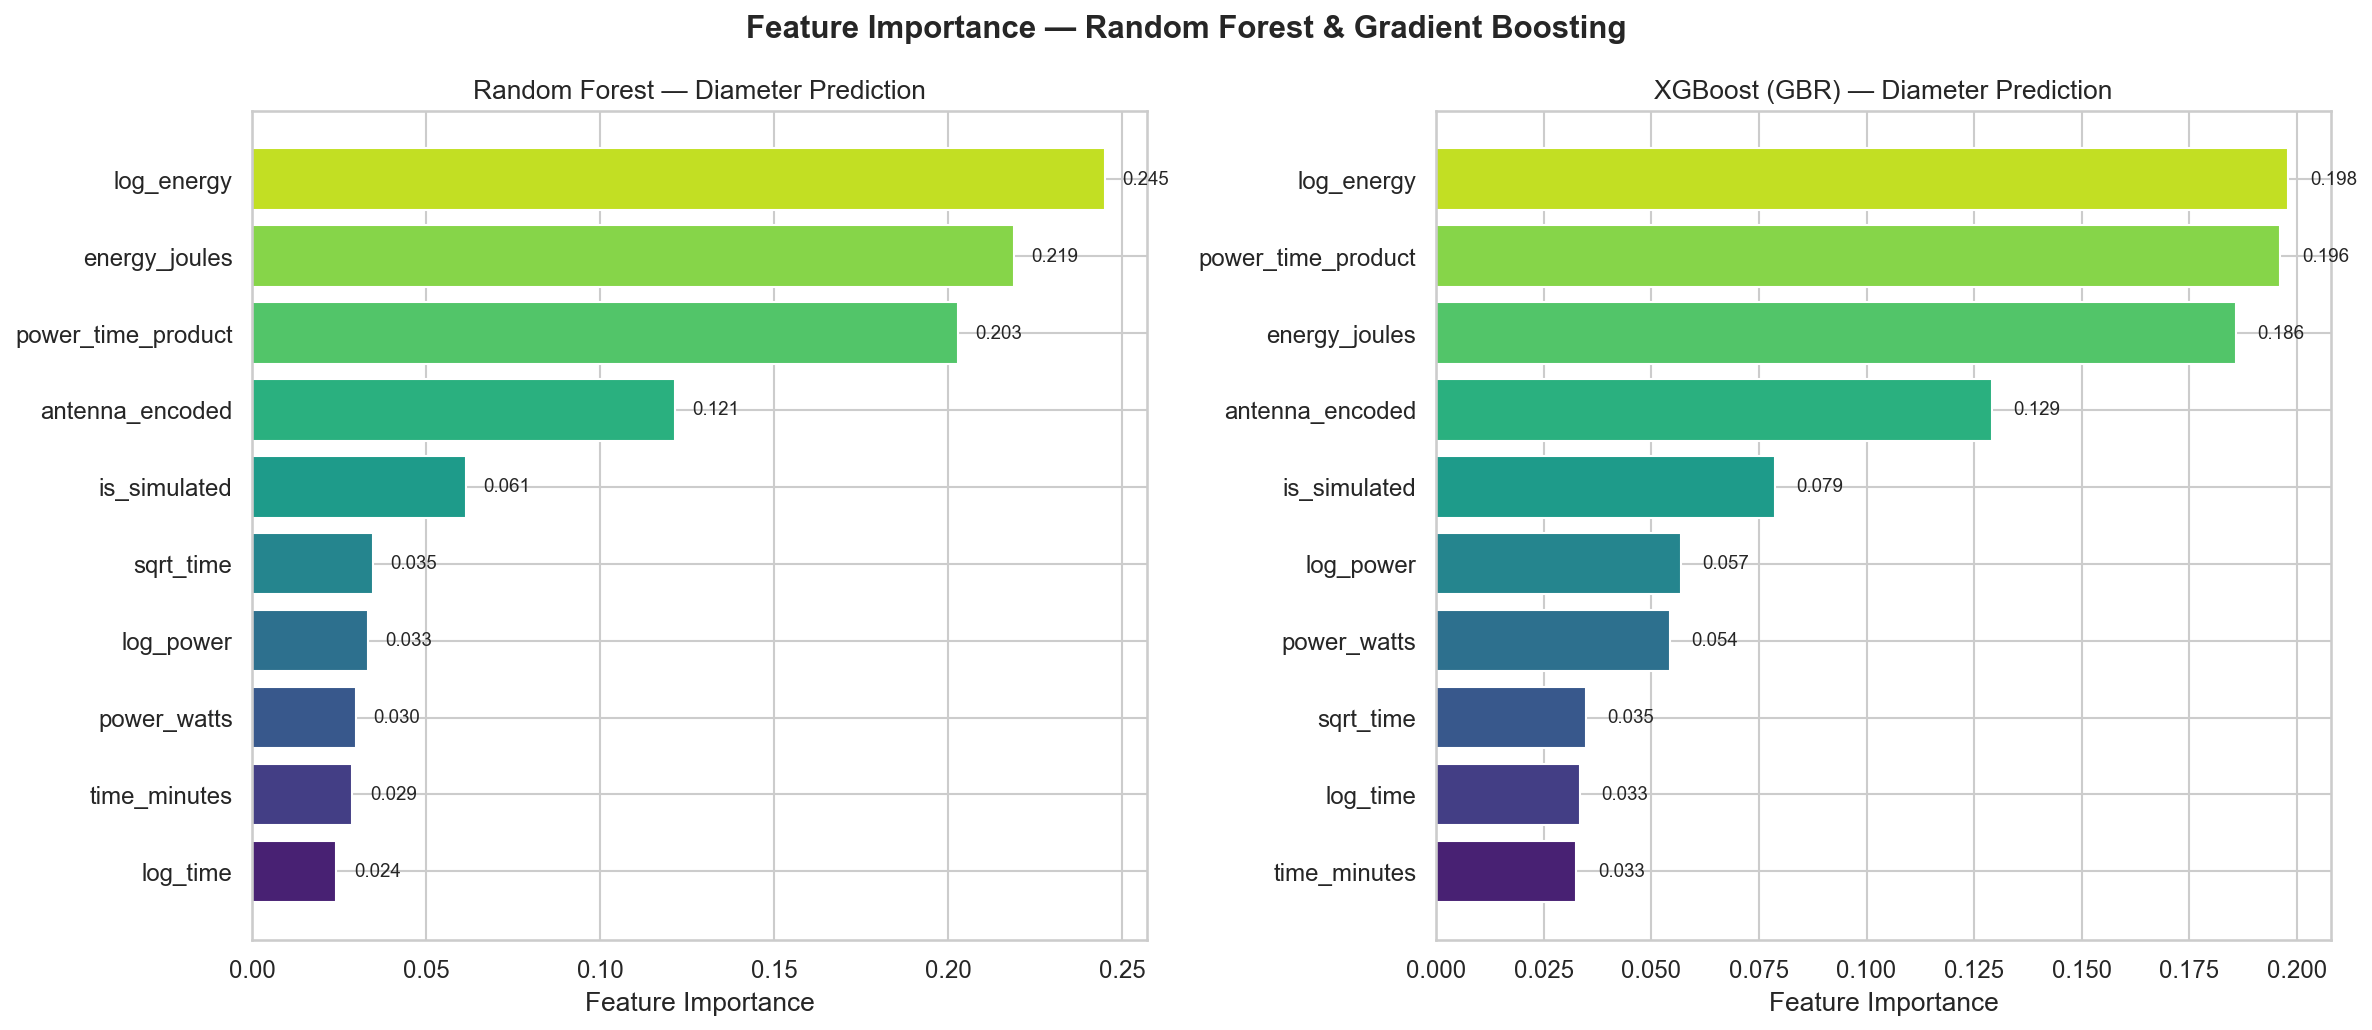
\includegraphics[width=0.85\textwidth]{feature_importance.png}
\caption{Feature importance from the Random Forest model for diameter prediction.}
\label{fig:feature-importance}
\end{figure}

Top features for diameter prediction (Random Forest):

\begin{table}[H]
\centering
\caption{Feature importance ranking for effective diameter prediction.}
\label{tab:feature-importance}
\begin{tabular}{@{}clc@{}}
\toprule
\textbf{Rank} & \textbf{Feature} & \textbf{Importance} \\
\midrule
1 & \texttt{log\_energy}          & 0.2450 (24.5\%) \\
2 & \texttt{energy\_joules}       & 0.2190 (21.9\%) \\
3 & \texttt{power\_time\_product} & 0.2028 (20.3\%) \\
4 & \texttt{antenna\_encoded}     & 0.1214 (12.1\%) \\
5 & \texttt{is\_simulated}        & 0.0613 (6.1\%)  \\
\bottomrule
\end{tabular}
\end{table}

\textbf{Key insight}: Energy-related features (\texttt{log\_energy}, \texttt{energy\_joules}, \texttt{power\_time\_product}) collectively account for \textbf{66.7\%} of the prediction power, confirming that the total energy delivered is the dominant factor in determining ablation zone size. The antenna type contributes 12.1\%, highlighting that antenna design plays a meaningful but secondary role.

\subsection{Overfitting Analysis}
\label{sec:overfitting}

\begin{figure}[H]
\centering
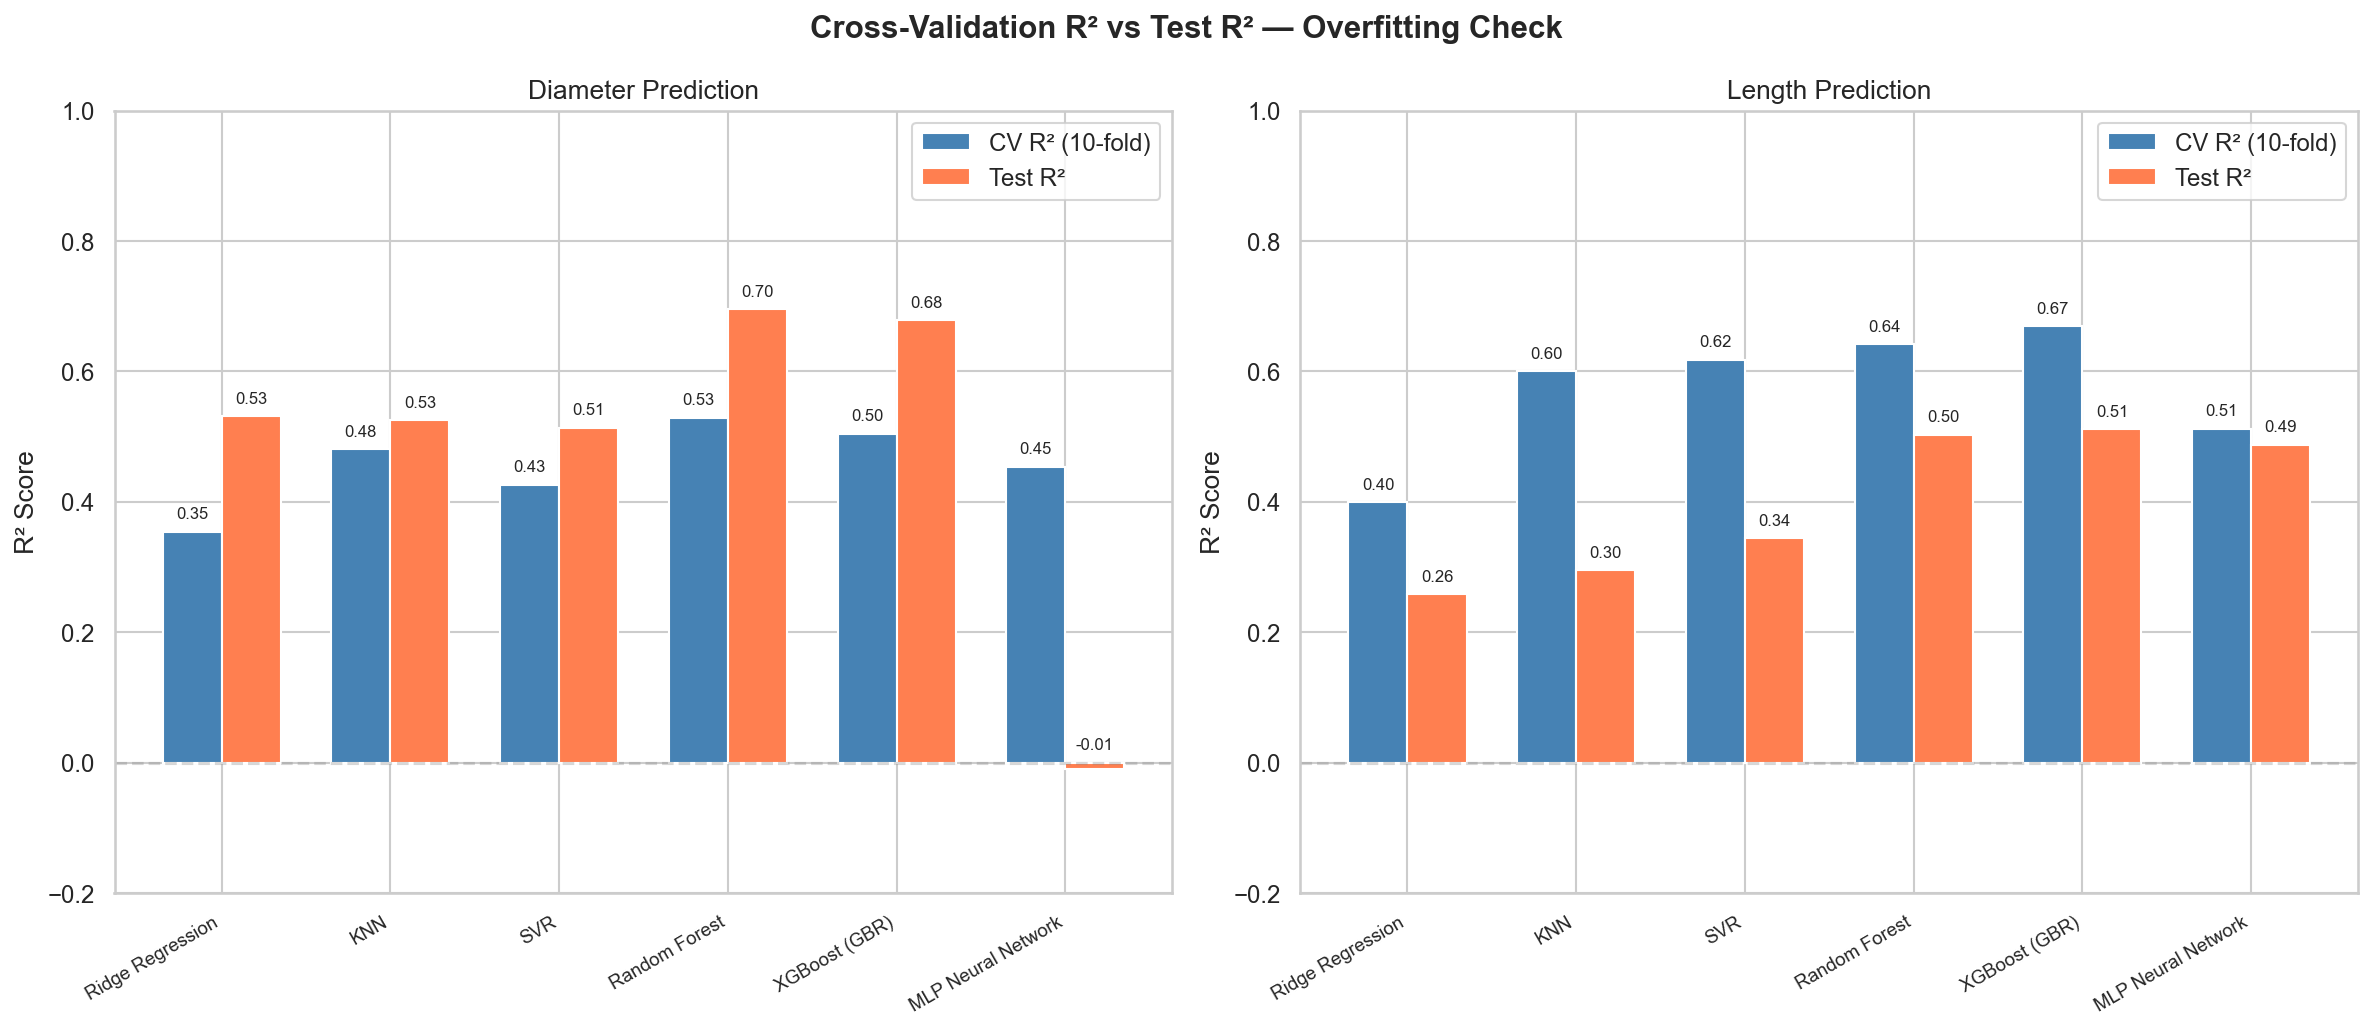
\includegraphics[width=0.85\textwidth]{cv_vs_test_comparison.png}
\caption{Cross-validation $R^2$ vs.\ test set $R^2$ for each model.}
\label{fig:cv-vs-test}
\end{figure}

Comparing cross-validation $R^2$ and test $R^2$ reveals:
\begin{itemize}
    \item \textbf{Random Forest (Diameter)}: CV $R^2 = 0.529$ vs.\ Test $R^2 = 0.695$ --- test performance is higher, suggesting the model generalizes well and may benefit from more training data.
    \item \textbf{KNN (Length)}: CV $R^2 = 0.601$ vs.\ Test $R^2 = 0.295$ --- significant drop, indicating overfitting to the training data.
    \item \textbf{MLP (Diameter)}: CV $R^2 = 0.454$ vs.\ Test $R^2 = -0.010$ --- severe overfitting; the neural network failed to generalize with this dataset size.
\end{itemize}

\subsection{Discussion}
\label{sec:discussion}

\textbf{Why Tree-Based Models Perform Best:}
\begin{enumerate}
    \item \textbf{Tabular data}: Random Forest and Gradient Boosting are consistently the top performers on structured tabular data, as confirmed by large-scale benchmarking studies.
    \item \textbf{Small dataset}: With only $\sim$230 training samples, tree ensembles' built-in regularization (bagging for RF, shallow trees for GBR) prevents overfitting.
    \item \textbf{Mixed feature types}: Trees naturally handle the combination of continuous features (power, time) and categorical features (antenna type).
    \item \textbf{Non-linear relationships}: The relationship between treatment parameters and ablation zone size is inherently non-linear (saturation effects, thermal diffusion).
\end{enumerate}

\textbf{Why MLP Underperformed:}\\
The neural network suffered from overfitting despite regularization (early stopping, weight decay). With only 233 training samples, the network could not learn robust representations, leading to a negative $R^2$ on the test set for diameter prediction.

% ═════════════════════════════════════════════════════════════
\section{Prediction Demo System}
\label{sec:demo}

\subsection{System Design}
\label{sec:system-design}

An interactive command-line prediction system was built using the best trained models. The system accepts clinical parameters and outputs predicted ablation zone dimensions in real-time.

\textbf{Input Parameters:}
\begin{itemize}
    \item Power (Watts)
    \item Time (minutes)
    \item Antenna category (from 15 types)
\end{itemize}

\textbf{Output Predictions:}
\begin{itemize}
    \item Effective diameter (mm)
    \item Length (mm)
    \item Estimated volume (mm$^3$) --- computed as an ellipsoid:
    \begin{equation}
        V = \frac{4}{3}\,\pi\,\frac{L}{2}\,\left(\frac{D}{2}\right)^2
    \end{equation}
    \item Sphericity index --- $D/L$ ratio
\end{itemize}

\subsection{Sample Predictions}
\label{sec:sample-predictions}

\begin{table}[H]
\centering
\caption{Sample predictions from the demo system.}
\label{tab:sample-predictions}
\begin{tabular}{@{}cccccc@{}}
\toprule
\textbf{Power (W)} & \textbf{Time (min)} & \textbf{Antenna} & \textbf{Pred.\ Diameter (mm)} & \textbf{Pred.\ Length (mm)} & \textbf{Est.\ Volume (mm$^3$)} \\
\midrule
50  & 5  & Dual Slot & $\sim$27 & $\sim$38 & $\sim$14\,500 \\
50  & 10 & Dual Slot & $\sim$33 & $\sim$47 & $\sim$26\,800 \\
100 & 5  & Monopole  & $\sim$35 & $\sim$50 & $\sim$32\,000 \\
100 & 10 & Monopole  & $\sim$42 & $\sim$58 & $\sim$53\,500 \\
20  & 5  & Dipole    & $\sim$20 & $\sim$30 & $\sim$6\,300  \\
80  & 10 & Triaxial  & $\sim$38 & $\sim$45 & $\sim$34\,000 \\
\bottomrule
\end{tabular}
\end{table}

These predictions align with published experimental data, demonstrating the model's practical utility for treatment planning.

% ═════════════════════════════════════════════════════════════
\section{Conclusion \& Future Work}
\label{sec:conclusion}

\subsection{Conclusion}
\label{sec:conclusion-summary}

This project successfully developed an AI/ML-based predictive model for microwave ablation zone estimation. Key outcomes include:

\begin{enumerate}
    \item \textbf{A curated dataset} of 326 samples from 30+ published studies was created, spanning experimental and simulation data across 15 antenna types.
    \item \textbf{Comprehensive feature engineering} extracted meaningful numerical features from unstructured text, including energy-based and log-transformed features.
    \item \textbf{Six ML models} were trained and compared using 10-fold cross-validation and GridSearchCV.
    \item \textbf{Random Forest} emerged as the best model for diameter prediction ($R^2 = 0.695$, MAE $= 6.02$\,mm), while \textbf{Gradient Boosting} performed best for length prediction ($R^2 = 0.512$, MAE $= 10.93$\,mm).
    \item \textbf{Energy delivered} (power $\times$ time) was identified as the single most important predictor of ablation zone size, accounting for $\sim$67\% of feature importance.
    \item An \textbf{interactive prediction system} was built for real-time ablation zone estimation.
\end{enumerate}

The model achieves clinically meaningful accuracy --- a MAE of 6\,mm for diameter prediction is within the range of measurement uncertainty in published studies --- and runs in milliseconds compared to hours for physics-based simulations.

\subsection{Limitations}
\label{sec:limitations}

\begin{enumerate}
    \item \textbf{Dataset size}: 326 samples is small for ML; more data would improve generalization.
    \item \textbf{Missing features}: Antenna-specific parameters (length, slot dimensions, frequency) were not consistently available and could improve accuracy.
    \item \textbf{Tissue variability}: The dataset combines different tissue types (liver, lung, kidney, egg white, bovine) without tissue-type encoding.
    \item \textbf{Temperature data}: Only 29.1\% of entries had temperature data, limiting its use as a feature.
    \item \textbf{Heterogeneous sources}: Data aggregated from multiple papers may have measurement biases.
\end{enumerate}

\subsection{Future Work}
\label{sec:future-work}

\begin{enumerate}
    \item \textbf{Expand the dataset} with more recent publications and additional ablation modalities.
    \item \textbf{Include tissue-specific features} (perfusion rate, dielectric properties, tissue type).
    \item \textbf{Deep learning approaches} with larger datasets (e.g., physics-informed neural networks).
    \item \textbf{3D ablation zone shape prediction} using image-based ML models.
    \item \textbf{Web-based clinical tool} with a user-friendly interface for treatment planning.
    \item \textbf{Multi-output models} that simultaneously predict diameter, length, and volume.
\end{enumerate}

% ═════════════════════════════════════════════════════════════
\section{References}
\label{sec:references}

\begin{enumerate}[label={[\arabic*]}]
    \item Dual-slot antennas for microwave tissue heating: Parametric design analysis and experimental validation (2011). \textit{Medical Physics}.

    \item A Minimally Invasive Antenna for Microwave Ablation Therapies: Design, Performances, and Experimental Assessment (2011). \textit{IEEE Transactions on Biomedical Engineering}.

    \item Heating characteristics of antenna arrays used in microwave ablation: A theoretical parametric study (2013). \textit{International Journal of Hyperthermia}.

    \item Antenna design and tissue parameters considerations for an improved modelling of microwave ablation in the liver (2013). \textit{Physics in Medicine and Biology}.

    \item Microwave Ablation at 10.0 GHz Achieves Comparable Ablation Zones to 1.9 GHz in Ex Vivo Bovine Liver (2014). \textit{Journal of Vascular and Interventional Radiology}.

    \item Optimization of dual slot antenna using floating metallic sleeve for microwave ablation (2014). \textit{Bioelectromagnetics}.

    \item Microwave ablation at 915 MHz vs 2.45 GHz: A theoretical and experimental investigation (2015). \textit{Medical Engineering \& Physics}.

    \item Analysis of minimally invasive directional antennas for microwave tissue ablation (2016). \textit{International Journal of Hyperthermia}.

    \item Analysis of microwave ablation antenna optimization techniques (2017). \textit{International Journal of RF and Microwave Computer-Aided Engineering}.

    \item A Minimally Invasive Coax-Fed Microwave Ablation Antenna With a Tapered Balun (2017). \textit{IEEE Transactions on Antennas and Propagation}.

    \item Non-coaxial-based microwave ablation antennas for creating symmetric and asymmetric coagulation zones (2018). \textit{Medical Engineering \& Physics}.

    \item Microwave antennas for thermal ablation of benign adrenal adenomas (2019). \textit{Biomedical Physics \& Engineering Express}.

    \item Toward Flexible Microwave Ablation Antennas With a Balun-Free Helical Dipole Design (2020). \textit{IEEE Transactions on Biomedical Engineering}.

    \item Triple Coaxial-Half-Slot Antenna Scheme With Deep Learning-Based Temperature Prediction for Hepatic Microwave Ablation (2021). \textit{IEEE Access}.

    \item A Minimally Invasive Microwave Ablation Antenna With Highly Localized Ablation Zone (2022). \textit{IEEE Transactions on Biomedical Engineering}.

    \item Feasibility Study of Microsecond Pulsed Microwave Ablation Using a Minimally Invasive Antenna (2022). \textit{IEEE Journal of Electromagnetics, RF and Microwaves in Medicine and Biology}.

    \item Microwave Antenna Design for Cardiovascular Applications (2023). \textit{Bioengineering}.

    \item A Flexible Microwave Ablation Antenna for Lung Cancer Treatment (2023). \textit{Scientific Reports}.

    \item Design of Microwave Ablation Antenna for Flexible Omnidirectional/Directional Ablation Zone Control (2025). \textit{IEEE Transactions on Biomedical Engineering}.

    \item Multi-Objective Optimization Design and Numerical Study of Water-Cooled Microwave Ablation Antennas (2025). \textit{Biomedical Engineering Letters}.
\end{enumerate}

\end{document}
